%  LaTeX support: latex@mdpi.com 
%  For support, please attach all files needed for compiling as well as the log file, and specify your operating system, LaTeX version, and LaTeX editor.

%=================================================================
\documentclass[cancers,article,submit,moreauthors,pdftex]{Definitions/mdpi}
\maxdeadcycles=300 % Output loop---200 consecutive dead cycles.

% For posting an early version of this manuscript as a preprint, you may use "preprints" as the journal and change "submit" to "accept". The document class line would be, e.g., \documentclass[preprints,article,accept,moreauthors,pdftex]{mdpi}. This is especially recommended for submission to arXiv, where line numbers should be removed before posting. For preprints.org, the editorial staff will make this change immediately prior to posting.

%--------------------
% Class Options:
%--------------------
%----------
% journal
%----------
% Choose between the following MDPI journals:
% acoustics, actuators, addictions, admsci, adolescents, aerospace, agriculture, agriengineering, agronomy, ai, algorithms, allergies, analytica, animals, antibiotics, antibodies, antioxidants, appliedchem, applmech, applmicrobiol, applnano, applsci, arts, asi, atmosphere, atoms, audiolres, automation, axioms, batteries, bdcc, behavsci, beverages, biochem, bioengineering, biologics, biology, biomechanics, biomedicines, biomedinformatics, biomimetics, biomolecules, biophysica, biosensors, biotech, birds, bloods, brainsci, buildings, businesses, cancers, carbon, cardiogenetics, catalysts, cells, ceramics, challenges, chemengineering, chemistry, chemosensors, chemproc, children, civileng, cleantechnol, climate, clinpract, clockssleep, cmd, coatings, colloids, compounds, computation, computers, condensedmatter, conservation, constrmater, cosmetics, crops, cryptography, crystals, curroncol, cyber, dairy, data, dentistry, dermato, dermatopathology, designs, diabetology, diagnostics, digital, disabilities, diseases, diversity, dna, drones, dynamics, earth, ebj, ecologies, econometrics, economies, education, ejihpe, electricity, electrochem, electronicmat, electronics, encyclopedia, endocrines, energies, eng, engproc, entropy, environments, environsciproc, epidemiologia, epigenomes, fermentation, fibers, fire, fishes, fluids, foods, forecasting, forensicsci, forests, fractalfract, fuels, futureinternet, futuretransp, futurepharmacol, futurephys, galaxies, games, gases, gastroent, gastrointestdisord, gels, genealogy, genes, geographies, geohazards, geomatics, geosciences, geotechnics, geriatrics, hazardousmatters, healthcare, hearts, hemato, heritage, highthroughput, histories, horticulturae, humanities, hydrogen, hydrology, hygiene, idr, ijerph, ijfs, ijgi, ijms, ijns, ijtm, ijtpp, immuno, informatics, information, infrastructures, inorganics, insects, instruments, inventions, iot, j, jcdd, jcm, jcp, jcs, jdb, jfb, jfmk, jimaging, jintelligence, jlpea, jmmp, jmp, jmse, jne, jnt, jof, joitmc, jor, journalmedia, jox, jpm, jrfm, jsan, jtaer, jzbg, kidney, land, languages, laws, life, liquids, literature, livers, logistics, lubricants, machines, macromol, magnetism, magnetochemistry, make, marinedrugs, materials, materproc, mathematics, mca, measurements, medicina, medicines, medsci, membranes, metabolites, metals, metrology, micro, microarrays, microbiolres, micromachines, microorganisms, minerals, mining, modelling, molbank, molecules, mps, mti, nanoenergyadv, nanomanufacturing, nanomaterials, ncrna, network, neuroglia, neurolint, neurosci, nitrogen, notspecified, nri, nursrep, nutrients, obesities, oceans, ohbm, onco, oncopathology, optics, oral, organics, osteology, oxygen, parasites, parasitologia, particles, pathogens, pathophysiology, pediatrrep, pharmaceuticals, pharmaceutics, pharmacy, philosophies, photochem, photonics, physchem, physics, physiolsci, plants, plasma, pollutants, polymers, polysaccharides, proceedings, processes, prosthesis, proteomes, psych, psychiatryint, publications, quantumrep, quaternary, qubs, radiation, reactions, recycling, regeneration, religions, remotesensing, reports, reprodmed, resources, risks, robotics, safety, sci, scipharm, sensors, separations, sexes, signals, sinusitis, smartcities, sna, societies, socsci, soilsystems, solids, sports, standards, stats, stresses, surfaces, surgeries, suschem, sustainability, symmetry, systems, taxonomy, technologies, telecom, textiles, thermo, tourismhosp, toxics, toxins, transplantology, traumas, tropicalmed, universe, urbansci, uro, vaccines, vehicles, vetsci, vibration, viruses, vision, water, wevj, women, world 

%---------
% article
%---------
% The default type of manuscript is "article", but can be replaced by: 
% abstract, addendum, article, book, bookreview, briefreport, casereport, comment, commentary, communication, conferenceproceedings, correction, conferencereport, entry, expressionofconcern, extendedabstract, datadescriptor, editorial, essay, erratum, hypothesis, interestingimage, obituary, opinion, projectreport, reply, retraction, review, perspective, protocol, shortnote, studyprotocol, systematicreview, supfile, technicalnote, viewpoint, guidelines, registeredreport, tutorial
% supfile = supplementary materials

%----------
% submit
%----------
% The class option "submit" will be changed to "accept" by the Editorial Office when the paper is accepted. This will only make changes to the frontpage (e.g., the logo of the journal will get visible), the headings, and the copyright information. Also, line numbering will be removed. Journal info and pagination for accepted papers will also be assigned by the Editorial Office.

%------------------
% moreauthors
%------------------
% If there is only one author the class option oneauthor should be used. Otherwise use the class option moreauthors.

%---------
% pdftex
%---------
% The option pdftex is for use with pdfLaTeX. If eps figures are used, remove the option pdftex and use LaTeX and dvi2pdf.

%%%%%%%%%%%%%%%%%%%%%%%%%%%%%%%%%% Tex
\usepackage[]{caption} % bf
\newcommand{\bcaption}[2]{\caption{\textbf{#1} #2}}
\usepackage{outlines}
% mark in blue or red
\usepackage{xcolor}

\newenvironment{MyColorPar}[1]{%
    \leavevmode\color{#1}\ignorespaces%
}{%
}%
%\usepackage[upplemac]{inputenc} %applemac support if unicode package fails
%\usepackage[latin1]{inputenc} %UNIX support if unicode package fails
%...
%\usepackage{graphicx}
%\DeclareGraphicsExtensions{.pdf,.png} % for high-resolution PDF image
%\usepackage{hyperref}
%\usepackage{url}

\usepackage{array}
\usepackage{ragged2e}
\usepackage{rotating}
\usepackage{tabularx}
\usepackage{makecell}
% \usepackage{array}
\usepackage{multirow}
\usepackage{colortbl}
\usepackage{hhline}
\usepackage{siunitx} % for  1e-10 scientific notation
%\usepackage{caption}
%\usepackage{subcaption}
\usepackage{booktabs, multirow} % for borders and merged ranges
\usepackage{soul}% for underlines
%\usepackage[table]{xcolor} % for cell colors
\usepackage{changepage,threeparttable} 

%%% for abbreviations, or acronyms
\usepackage[automake, acronym, nopostdot]{glossaries} 
\usepackage{glossary-inline}
%\setacronymstyle{long-short}
%\renewcommand*{\glossarysection}[2][]{} 
%\renewcommand*{\glossarysection}[2][]{\textbf{#1}: }
% for abbreviations environment
%\newcommand{\abbrlabel}[1]{\makebox[3cm][l]{\textbf{#1}\ \dotfill}}
\newenvironment{abbreviation}%{\begin{list}{}{\renewcommand{\makelabel}{\abbrlabel}}}{\end{list}}
% \newenvironment{<name>}[<number>][<default>]


\makeglossaries %https://tex.stackexchange.com/questions/110095/list-of-acronyms-is-not-displayed
\newacronym{fdr}{FDR}{false discovery rate}

\newacronym{hpa}{HPA}{the Human Protein Atlas}
\newacronym{hnscc}{HNSCC}{head and neck squamous cell carcinoma}
\newacronym{tcga}{TCGA}{the Cancer Genome Atlas}
\newacronym{tcpa}{TCPA}{the Cancer Proteome Atlas}
\newacronym{rna}{RNA}{ribonucleic acid}
\newacronym{rnaseq}{RNA-Seq}{RNA sequencing}
\newacronym{lncrna}{lncRNA}{long non-coding RNA}
%\newacronym{km}{KM}{Kaplan-Meier}
\newacronym{rppa}{RPPAs}{reverse-phase protein arrays}
\newacronym{rpma}{RPMA}{reverse-phase protein lysate microarray}

\newacronym{mmp}{MMP}{matrix metalloproteinase}
 %DKK1, CAMK2N1, STC2, PGK1, SURF4, USP10, NDFIP1, FOXA2, STIP1, and DKC1
 %ZNF557, ZNF266, IL19, MYO1H, FCGBP, LOC148709, EVPLL, PNMA5, KIAA1683, and NPB

\newacronym{DKK1}{DKK1}{dickkopf WNT signaling pathway inhibitor 1} 
\newacronym{CAMK2N1}{CAMK2N1}{calcium/calmodulin dependent protein kinase II inhibitor 1} 
\newacronym{STC2}{STC2}{stanniocalcin 2} 
\newacronym{PGK1}{PGK1}{phosphoglycerate kinase 1} 
\newacronym{SURF4}{SURF4}{surfeit 4} 
\newacronym{USP10}{USP10}{ubiquitin specific peptidase 10} 
\newacronym{NEDD4}{NEDD4}{neural precursor cell expressed, developmentally down-regulated 4}
\newacronym{NDFIP1}{NDFIP1}{NEDD4 family interacting protein 1} 
\newacronym{FOXA2}{FOXA2}{forkhead box A2} 
\newacronym{STIP1}{STIP1}{stress-induced-phosphoprotein 1} 
\newacronym{DKC1}{DKC1}{dyskeratosis congenita 1, dyskerin} 

\newacronym{ZNF557}{ZNF557}{zinc finger protein 557} 
\newacronym{ZNF266}{ZNF266}{zinc finger protein 266} 
\newacronym{IL19}{IL19}{interleukin 19} 
\newacronym{MYO1H}{MYO1H}{myosin 1H} 
\newacronym{FCGBP}{FCGBP}{Fc fragment of IgG binding protein} 
\newacronym{LOC148709}{LOC148709}{LncRNA LOC148709} 
\newacronym{EVPLL}{EVPLL}{envoplakin-like protein} 
\newacronym{PNMA5}{PNMA5}{paraneoplastic antigen like 5} 
%\newacronym{KIAA1683}{KIAA1683}{IQCN, IQ Motif Containing N} 
\newacronym{IQCN}{IQCN}{IQ motif containing N} % previous name KIAA1683
% "IQ" refers to the first two amino acids of the motif: isoleucine (commonly) and glutamine (invariably)
\newacronym{NPB}{NPB}{neuropeptide B} 

 \newacronym{rt}{RT}{radiation therapy}
 \newacronym{nccn}{NCCN}{National Comprehensive Cancer Network}
 \newacronym{hif}{HIF}{hypoxia-inducible factor}
 \newacronym{egfr}{EGFR}{epidermal growth factor receptor}
 \newacronym{ras}{RAS}{rat sarcoma}
 \newacronym{hras}{HRAS}{Harvey rat sarcoma viral oncoprotein}
 \newacronym{erk}{ERK}{extracellular signal-regulated kinases}
 \newacronym{us}{US}{United States}
 \newacronym{fda}{FDA}{Food and Drug Administration}
 \newacronym{tpf}{Tax-PF}{docetaxel, cisplatin, and 5-fluorouracil}
 \newacronym{tki}{TKI}{tyrosine kinase inhibitor}
 \newacronym{her}{HER}{human epidermal growth factor receptor}
 \newacronym{ici}{ICI}{immune-checkpoint inhibitor}
 \newacronym{ctla4}{CTLA-4}{cytotoxic T lymphocyte antigen 4}
 \newacronym{pd1}{PD-1}{programmed death 1}
 \newacronym{pdl1}{PD-L1}{programmed death ligand 1}
 \newacronym{tim3}{TIM-3}{T-cell immunoglobulin mucin protein 3}
 \newacronym{lag3}{LAG-3}{lymphocyte activation gene 3}
 \newacronym{ifng}{IFN-$\gamma$}{interferon gamma}
 \newacronym{tigit}{TIGIT}{T cell immunoglobin and immunoreceptor tyrosine-based inhibitory motif}
 \newacronym{gitr}{GITR}{glucocorticoid-induced tumor necrosis factor receptor}
 \newacronym{vista}{VISTA}{V-domain Ig suppressor of T-cell activation}
 \newacronym{tmsb4x}{TMSB4X}{thymosin beta-4 X-linked}
 \newacronym{emt}{EMT}{epithelial-mesenchymal-transition}
 \newacronym{gdc}{GDC}{Genomic Data Commons}
 \newacronym{nci}{NCI}{the National Cancer Institute}
 \newacronym{gdac}{GDAC}{Genome Data Analysis Center}
 \newacronym{rest}{REST}{Representational State Transfer} 
 \newacronym{api}{API}{Application Programmable Interface}
\newacronym{grch38}{GRCh38}{Genome Reference Consortium Homo sapiens genome assembly 38}
\newacronym{fpkm}{FPKM}{Fragments per kilobase per million reads mapped}
\newacronym{rsem}{RSEM}{RNA-Seq by Expectation-Maximization}
\newacronym{slca}{SLC35E2A}{solute carrier family 35 member E2A}
\newacronym{slcb}{SLC35E2B}{solute carrier family 35 member E2B}
\newacronym{cde}{CDE}{Common Data Element}
\newacronym{id}{ID}{identification}
\newacronym{ajcc}{AJCC}{the American Joint Committee on Cancer}
\newacronym{uicc}{UICC}{he Union for International Cancer Control}
\newacronym{tnm}{TNM}{the tumor size (T), cervical lymph node metastases (N), and distal metastasis status (M)}
\newacronym{ci95}{95\% CI}{95\% confidence interval}
\newacronym{os}{OS}{overall survival}
\newacronym{hr}{HR}{hazard ratio}
\newacronym{hpv}{HPV}{human papillomavirus}
\newacronym{ene}{ENE}{extra-nodal extension}
\newacronym{lvsi}{LVSI}{lymph-vascular space invasion}
\newacronym{pni}{PNI}{perineural invasion}
\newacronym{doi}{DOI}{depth of invasion}
\newacronym{lnd}{LND}{lymph node density}
\newacronym{wpoi5}{WPOI-5}{worst pattern of invasion score 5}
\newacronym{glut4}{GLUT4}{glucose transporters 4}
\newacronym{slc2a4}{SLC2A4}{solute carrier family 2 member A4}
\newacronym{trim24}{TRIM24}{tripartite motif-containing 24}
\newacronym{til}{TIL}{tumor-infiltrating lymphocytes}
\newacronym{tmb}{TMB}{tumor mutational burden}


%=================================================================
\firstpage{1} 
\makeatletter 
\setcounter{page}{\@firstpage} 
\makeatother
\pubvolume{1}
\issuenum{1}
\articlenumber{0}
\pubyear{2021}
\copyrightyear{2021}
%\externaleditor{Academic Editor: Firstname Lastname}
\datereceived{} 
\dateaccepted{} 
\datepublished{} 

%------------------------------------------------------------------
% The following line should be uncommented if the LaTeX file is uploaded to arXiv.org
%\pdfoutput=1

%=================================================================
% Add packages and commands here. The following packages are loaded in our class file: fontenc, inputenc, calc, indentfirst, fancyhdr, graphicx, epstopdf, lastpage, ifthen, lineno, float, amsmath, setspace, enumitem, mathpazo, booktabs, titlesec, etoolbox, tabto, xcolor, soul, multirow, microtype, tikz, totcount, changepage, paracol, attrib, upgreek, cleveref, amsthm, hyphenat, natbib, hyperref, footmisc, url, geometry, newfloat, caption

%=================================================================
%% Please use the following mathematics environments: Theorem, Lemma, Corollary, Proposition, Characterization, Property, Problem, Example, ExamplesandDefinitions, Hypothesis, Remark, Definition, Notation, Assumption
%% For proofs, please use the proof environment (the amsthm package is loaded by the MDPI class).

%=================================================================
% Full title of the paper (Capitalized)
\Title{A Global Genome-wide Scan with Optimal Cutoff Mining for Emerging Biomarkers in Head and Neck Squamous Cell Carcinoma}

% MDPI internal command: Title for citation in the left column
\TitleCitation{A Global Genome-wide Scan with Optimal Cutoff Mining for Emerging Biomarkers in Head and Neck Squamous Cell Carcinoma}

% Author Orchid ID: enter ID or remove command
\newcommand{\orcidauthorA}{0000-0002-4476-2600} % Add \orcidA{} behind the author's name
\newcommand{\orcidauthorB}{0000-0001-6497-4232} % Add \orcidB{} behind the author's name

% Authors, for the paper (add full first names)
\Author{
Li-Hsing Chi $^{1,2}$\orcidA{}, Alexander TH Wu $^{1}$,
Michael Hsiao $^{3}$*
and Yu-Chuan (Jack) Li $^{1,4}$*\orcidB{}}
%\Author{Firstname Lastname $^{1,\dagger,\ddagger}$\orcidA{}, Firstname Lastname $^{1,\ddagger}$ and Firstname Lastname $^{2,}$*}

% MDPI internal command: Authors, for metadata in PDF
\AuthorNames{Li-Hsing Chi, Alexander TH Wu, Michael Hsiao and Yu-Chuan (Jack) Li}

% MDPI internal command: Authors, for citation in the left column
\AuthorCitation{Chi, LH.; Wu, ATH.; Hsiao, M.; Li, YCJ.}

% Affiliations / Addresses (Add [1] after \address if there is only one affiliation.)
\address{%
$^{1}$ \quad The Ph.D. Program for Translational Medicine, College of Medical Science and Technology\unskip, 
    Taipei Medical University and Academia Sinica\unskip, Taipei\unskip, Taiwan\\
$^{2}$ \quad Division of Oral and Maxillofacial Surgery, Department of Dentistry\unskip,
    Taipei Medical University Hospital\unskip, Taipei\unskip, Taiwan\\
$^{3}$ \quad Genomics Research Center\unskip, 
    Academia Sinica\unskip, Taipei\unskip, Taiwan\\
$^{4}$ \quad Graduate Institute of Biomedical Informatics, College of Medical Science and Technology\unskip, Taipei Medical University\unskip, Taipei\unskip, Taiwan\\
}

% Contact information of the corresponding author
\corres{Correspondence: Hsiao: mhsiao@gate.sinica.edu.tw; Li: jaak88@gmail.com}
%(optional; include country code; if there are multiple corresponding authors, add author initials) +xx-xxxx-xxx-xxxx (F.L.)}

% Current address and/or shared authorship
%\firstnote{Current address: Affiliation 3} 
%\secondnote{These authors contributed equally to this work.}
% The commands \thirdnote{} till \eighthnote{} are available for further notes

%\simplesumm{} % Simple summary

%\conference{} % An extended version of a conference paper

% Abstract (Do not insert blank lines, i.e. \\) 
\abstract{The survival analysis of the Cancer Genome Atlas (TCGA) dataset is a well-known method to discover the gene expression-based prognostic biomarkers of head and neck squamous cell carcinoma (HNSCC). It is necessary to determine a cutoff point by the patients' dichotomization for the continuous gene expression in survival analysis. There is some optimization software for cutoff determination. However, the software's predetermined cutoffs are usually set at the median or quantiles of RNA sequencing value to perform the survival analyses. There are few clinicopathological features available on their pre-processed data sets.
We developed a comprehensive workflow that includes data retrieving and pre-processing, feature selection, cutoff mining engine, Kaplan-Meier survival analysis, Cox proportional hazard modeling, and biomarker discovery.
Using this workflow on the TCGA HNSCC cohort, we scanned human protein-coding genes. After adjustment with confounders and Bonferroni adjusted P-value, ten candidate biomarkers, named as DKK1, CAMK2N1, STC2, PGK1, SURF4, USP10, NDFIP1, FOXA2, STIP1, and DKC1, are significantly associated with the poor prognosis of overall survival. At the same time, the other ten genes were over-expressed in the better survival patients, named as ZNF557, ZNF266, IL19, MYO1H, FCGBP, LOC148709, EVPLL, PNMA5, IQCN (previous name as KIAA1683), and NPB.
We suggest this workflow could help for biomarker discovery.}

% Keywords
\keyword{Head and Neck Squamous Cell Carcinoma (HNSCC);
%Genome Database\sep
the Cancer Genome Atlas (TCGA);
RNA-sequencing;
Survival Analysis;
Optimal Cutoff;
%Biomarker\sep % Discovery\sep
%Tumor Type-agnostic Therapy\sep
%Immuno-Oncology\sep
%Targeted Therapy\sep
%Systemic Therapy\sep
Surgical Margin}


%%%%%%%%%%%%%%%%%%%%%%%%%%%%%%%%%%%%%%%%%%


\begin{document}
%\begin{paracol}{2}
%%%%%%%%%%%%%%%%%%%%%%%%%%%%%%%%%%%%%%%%%%
%\setcounter{section}{-1} %% Remove this when starting to work on the template.
%\section{How to Use this Template}

%The template details the sections that can be used in a manuscript. Note that the order and names of article sections may differ from the requirements of the journal (e.g., the positioning of the Materials and Methods section). Please check the instructions on the authors' page of the journal to verify the correct order and names. For any questions, please contact the editorial office of the journal or support@mdpi.com. For LaTeX-related questions please contact latex@mdpi.com.
%The order of the section titles is: Introduction, Materials and Methods, Results, Discussion, Conclusions for these journals: aerospace,algorithms,antibodies,antioxidants,atmosphere,axioms,biomedicines,carbon,crystals,designs,diagnostics,environments,fermentation,fluids,forests,fractalfract,informatics,information,inventions,jfmk,jrfm,lubricants,neonatalscreening,neuroglia,particles,pharmaceutics,polymers,processes,technologies,viruses,vision

\section{Introduction}

Head and neck squamous cell carcinoma (\acrshort{hnscc}), including oral, oropharyngeal, and hypopharyngeal origin, is the fourth leading cancer causes of death for males in Taiwan\cite{MOHW_death2017}. The age-standardized incidence rate of \acrshort{hnscc} in males is 42.43 per 100,000 persons\cite{MOHW_incidence2018}. 
% chemotherapy => systemic therapy
The treatment strategies of \acrshort{hnscc} are surgery alone, systemic therapy with concurrent radiation therapy (systemic therapy/\acrshort{rt}), or surgery with adjuvant systemic therapy/\acrshort{rt} (according to \acrlong{nccn}, \acrshort{nccn} Clinical Practice Guidelines in \acrshort{hnscc}, Version 2.2020)\cite{Pfister2020a}. Despite the improvement in those interventions, the survival of \acrshort{hnscc} has improved only marginally over the past decade worldwide\cite{hpa2019}. The critical advancement of targeted therapy and immuno-oncology should benefit from emerging prognostic biomarkers, which guide the development of modern systemic therapy.

%% TP53 gene => p53 protein; mutation of TP53
Accumulative knowledge showed that some biomarkers have prognostic significance in \acrshort{hnscc}. For example, node-negative \acrshort{hnscc} patients with p53 overexpression were found to have lower survival\cite{DeVicente2004}.
Overexpression of \acrfull{hif}-1 alpha\cite{Aebersold2001} or Ki-67\cite{Couture2002} was found to be correlated with poor response to radiotherapy of \acrshort{hnscc}. The \acrfull{egfr}\cite{O-Charoenrat2000}\cite{Bentzen2005} and \acrfull{mmp}\cite{Harrington2017} were found to be over-expressed to promote invasion and metastasis of \acrshort{hnscc}.
From 2000 to 2006, the anti-\acrshort{egfr} antibody-drug (cetuximab) has been developed and combined with radiotherapy, known as bio-\acrshort{rt}, to increase survival of unresectable locoregionally advanced disease\cite{Bonner2006a}.
The systemic therapy of cetuximab plus platinum-fluorouracil chemotherapy (EXTREME regimen) improves overall survival when given as first-line treatment in patients with recurrent or metastatic \acrshort{hnscc}\cite{Vermorken2008}\cite{Rivera2009}. It was approved by the \acrshort{us} \acrfull{fda} in 2008. In advance, the bio-\acrshort{rt} could have proceeded with \acrfull{tpf} induction chemotherapy to overcome the radio-resistance of \acrshort{hnscc}\cite{Blanchard2013}.

However, Rampias and his colleagues suggested \acrfull{hras} mutations could mediate cetuximab resistance in systemic therapy of \acrshort{hnscc} via the \acrshort{egfr}/\acrfull{ras}/\acrfull{erk} signaling pathway\cite{Rampias2014}.
After that, the \acrshort{egfr} \acrfull{tki} was introduced to help cetuximab in 2018. The anti-tumor activity was observed in a phase 1 trial for \acrshort{hnscc} patients using cetuximab and afatinib, a \acrshort{tki} of \acrshort{egfr}, \acrfull{her}2, and \acrshort{her}4\cite{Gazzah2018}. Other \acrshort{egfr} \acrshort{tki}, such as gefitinib, erlotinib, osimertinib, were also developed to treat advanced \acrshort{hnscc}.
Although 90\% of \acrshort{hnscc} has overexpression of \acrshort{egfr}, cetuximab has only 10\% to 20\% response rate on those patients. So far, cetuximab is still the only drug of choice with proven efficacy, which targeted the selected \acrshort{hnscc} patients\cite{Taberna2019}.

Until the immuno-oncology era, \acrfull{ici} was introduced since 2014 for treating \acrshort{hnscc}\cite{Seiwert2014}\cite{Swanson2015}.
The \acrshort{ici} works on immune checkpoint molecules, which including \acrfull{pd1}, \acrfull{ctla4}, \acrfull{tim3}, \acrfull{lag3}, \acrfull{tigit}, \acrfull{gitr} and \acrfull{vista}\cite{Mei2020}.
The \acrshort{us} \acrshort{fda} has approved the anti-\acrshort{pd1} agents, pembrolizumab, and nivolumab, as a monotherapy for the platinum-treated patients of recurrent or metastatic \acrshort{hnscc}\cite{Cramer2019}. However, because of the complexity of immune-tumor interaction, \acrshort{ici} has not to guarantee the response to \acrfull{pdl1} expressed \acrshort{hnscc}\cite{Swanson2015}.
According to the phase 3 KEYNOTE-048 study, \acrshort{pdl1} is a validated biomarker used in clinical guidance for candidate selection of pembrolizumab\cite{Burtness2019}\cite{Gavrielatou2020}.

In our previous proteomic study in 2017, \acrfull{tmsb4x} was reported to be related to tumor growth and metastasis of \acrshort{hnscc}\cite{Chi2017}. It was also found by the subsequent investigations that \acrshort{tmsb4x} engaged in tumor aggressiveness through \acrfull{emt} on pancreatic\cite{Zhang2008}, gastric\cite{Ryu2012}, colorectal\cite{Gemoll2015}, lung\cite{Huang2016}, ovarian\cite{Chu2019} and melanoma\cite{Makowiecka2019} cancers. Thus, it might be suggested that \acrshort{tmsb4x}  is possible for tumor type-agnostic therapy\cite{Yan2018} as a common biomarker crossing several types of cancer.
%TMSB4X proteins regulate intracellular signal transduction and has been proved to overexpress in various cancers, including colorectal, lung, gastric, pancreatic, and squamous cell cancers.\cite{Chi2017}
% https://doi.org/10.1038/s41598-017-09539-w



\begin{MyColorPar}{red}
%%%%%% revision1 added [TCGA] [2021/02/02]
The Cancer Genome Atlas (TCGA) project\cite{Weinstein2013} is developed and supervised by the National Cancer Institute's (NCI) Center for Cancer Genomics and the National Human Genome Research Institute (NHGRI), funded by the US government since 2005.
TCGA represents comprehensive genomics and clinic data from 84,392 patients among 33 major cancer types (data release 27.0 - Oct 29, 2020, available at https://www.cancer.gov/about-nci/organization/ccg/research/structural-genomics/tcga/studied-cancers).
%The Cancer Genome Atlas (TCGA): The TCGA consortium, which is a National Institute of Health (NIH) initiative, makes publicly available molecular and clinical information for more than 33 types of human cancers including exome (variant analysis), single nucleotide polymorphism (SNP), DNA methylation, transcriptome (mRNA), microRNA (miRNA) and proteome.
TCGA and other collaborated \acrfull{gdac} generated and analyzed DNA (mutation, copy number variation, methylation, simple nucleotide polymorphism, SNP), RNA (microarray, RNA-Seq, microRNA), and protein (reverse protein phased array) data derived from biospecimen. Sample types available at TCGA are primary solid tumors, recurrent solid tumors, blood-derived normal and tumor, metastatic, and solid tissue normal.  

The NCI's Genomic Data Commons (GDC, available at https://portal.\\gdc.cancer.gov/) receives, processes, and distributes genomic, clinical, and biospecimen data from TCGA database and other cancer research programs. The clinical features has been defined by \acrshort{tcga} \acrshort{gdc} data dictionary: \acrfull{cde}\cite{CDE2019}. The \acrshort{rnaseq} expression data has been harmonized and re-aligned against an official reference genome build (\acrlong{grch38}, \acrshort{grch38}).
%The old TCGA data portal (https://tcga-data.nci.nih.gov/docs/publications/tcga/) stops updating and all TCGA data was transferred to the GDC data portal .
\acrshort{tcga}, GDC and research community offer several computational tools to the public for facilitating cancer research. %There is three categories of tools to approach the TCGA data from GDC.
GDC Data Portal (available at https://portal.gdc.cancer.gov) is the official web-based TCGA data analysis tools. Other available web-based tools have been reviewed by Zhang et al.\cite{Zhang2019b} and 
Matthieu Foll (availalbe at https://github.com/IARCbioinfo/awesome-TCGA).
One of \acrshort{gdac}s, the Broad TCGA Data and Analyses (Broad GDAC), provides Firehose, a repository of the TCGA public-accessible Level 3 data and Level 4 analyses. Broad GDAC Firehose is an analytical infrastructure that analyses algorithms not performed by the GDC (e.x. GISTIC, MutSig2CV, correlation with clinical variables, mRNA clustering). 
A web-based version of Broad GDAC Firehose is Firebrowse (available at firebrowse.org, Version: 1.1.40, 2019-10-13).
%Python and UNIX bindings
%R bindings
Broad GDAC Firebrowse provides graphical tools like viewGene to explore expression levels and iCoMut to explore a mutation analysis of each TCGA disease. 

%Second, GDC data transfer tool (available at https://gdc.cancer.gov/access-data/gdc-data-transfer-tool) allows users to access the open or controlled data. %the GDC data model, data formats
% RESTful API

GDC \acrfull{api} is designed under the \acrfull{rest} architecture and provides accessibility to external users for programmatic access to the same functionality found through GDC Portals. Those functions include searching, viewing, submitting, and downloading subsets of data files, metadata, and annotations based on specific parameters. Moreover, if restricted data is requested, the user must provide a token along with the API call. This token can be downloaded directly from the GDC Portals. (courtesy of the National Cancer Institute)
Broad GDAC Firebrowse \acrshort{rest}ful \acrshort{api} could be accessed using an R package, FirebrowseR (available at https://github.com/mariodeng/FirebrowseR)\cite{Deng2017}.

% clinical
%We utilized FirebrowseR's function call, Samples.Clinical(cohort = "HNSC", format="csv"), to get all 81 clinical features (including pathological data, defined by \acrshort{tcga} \acrshort{gdc} data dictionary: \acrfull{cde}\cite{CDE2019}) of all 528 \acrshort{hnscc} patient.

% to summarize the advantages of its use.
The highlights of the advantages of applying the TCGA data for cancer research include:
\begin{outline}
\1  To the best of our knowledge, the TCGA database is the largest collection (cancer types and cohort size) of comprehensive genomics with survival data available in the field of cancer research so far. The whole-genome sequencing data has been harmonized across all GDACs. The basic demographic data is usually available on many databases. However, TCGA data has more comprehensive features, such as exposure to alcohol, asbestos, radioactive radon, tobacco smoking, or cigarettes.
\1  TCGA has a remarkable advantage for computational and life scientists who study cancer since useful web-tools and API are ready to analyze and visualize TCGA data. It might be getting help quickly from the research community for trouble-shooting.
\1  Many achievements of diagnoses, treatments, and prevention with the TCGA data have already been published and keep growing.\cite{Tomczak2015}
\end{outline}

\end{MyColorPar}
%%%%%% end of additional revision1

In summary, identifying predictive biomarkers for selecting standard-of-care or advanced systemic therapy\cite{Cristina2019} in \acrshort{hnscc} is crucial. 
However, there are three challenges of biomarker discovery from survival analysis, so far.
Firstly, although \acrshort{tcga} genomics data were harmonized, there is unclean data, including null expressed genes, which over 50\% of the cohort, should be manually investigated and cleaned.
Second, we need to find a way to determine candidates from the expression level of 20,500 human protein-coding genes\cite{Clamp2007}. Usually, the investigators should get the rationale or revelation of the genes of interest on a specific cancer type. They should upload those genes manually onto bioinformatics tools, such as SurvExpress (http://bioinformatica.mty.itesm.mx:8080/Biomatec/ \newline
SurvivaX.jsp\cite{Aguirre-Gamboa2013}, which has been lost since Oct/2019 and currently out of funds), analyze with \acrshort{tcga} cohort. After downloading the survival results, they could curate plots and tables carefully.
It is not possible to scan the whole human protein-coding genome in this way.
Third, we need to find an optimal cutpoint of those \acrshort{rna} expression data to maximize candidate mining coverage. The above mentioned online tools might set a cutpoint at the median, 1/4 quantile, or 3/4 quantile for subsequent analyses. There are several visualization software or R packages which deal with cutoff determination, such as Prognoscan\cite{Mizuno2009a}, Cutoff Finder\cite{Budczies2012}, Findcut\cite{Chang2017a}, Human protein atlas\cite{Uhlen2017}, OptimalCutpoints\cite{Cristina2019},  cutpointr (available at https://github.com/thie1e/ \newline
cutpointr), and cutoffR (available at https://cran.r-project.org/web/
packages/cutoffR). However, non of them could combine the scanning of the protein-coding genes and cutoff optimization programmatically.

In our approach, this article described a comprehensive workflow implemented in the R script, which runs on the Rstudio server. Its functions include data retrieving and pre-processing, feature selection, cutoff mining engine, Kaplan-Meier survival analysis, Cox proportional hazard modeling, and biomarker selection.
Using this workflow on the \acrshort{tcga} \acrshort{hnscc} cohort, the 20,500 human protein-coding genes were scanned. The analysis workflow is shown in Figure \ref{fig:figure1}.
%We found that the surgical margin status and tobacco exposure are independent risk factors of patient survival. 
%Our findings also suggested several candidate biomarkers are associated with the prognosis of overall survival (OS) under optimal cutoff point with significant P-value. Those genes may be potential therapeutic targets of HNSCC.

%\subsubsection{Figure 1:h}
\begin{figure}[hp]
\centering
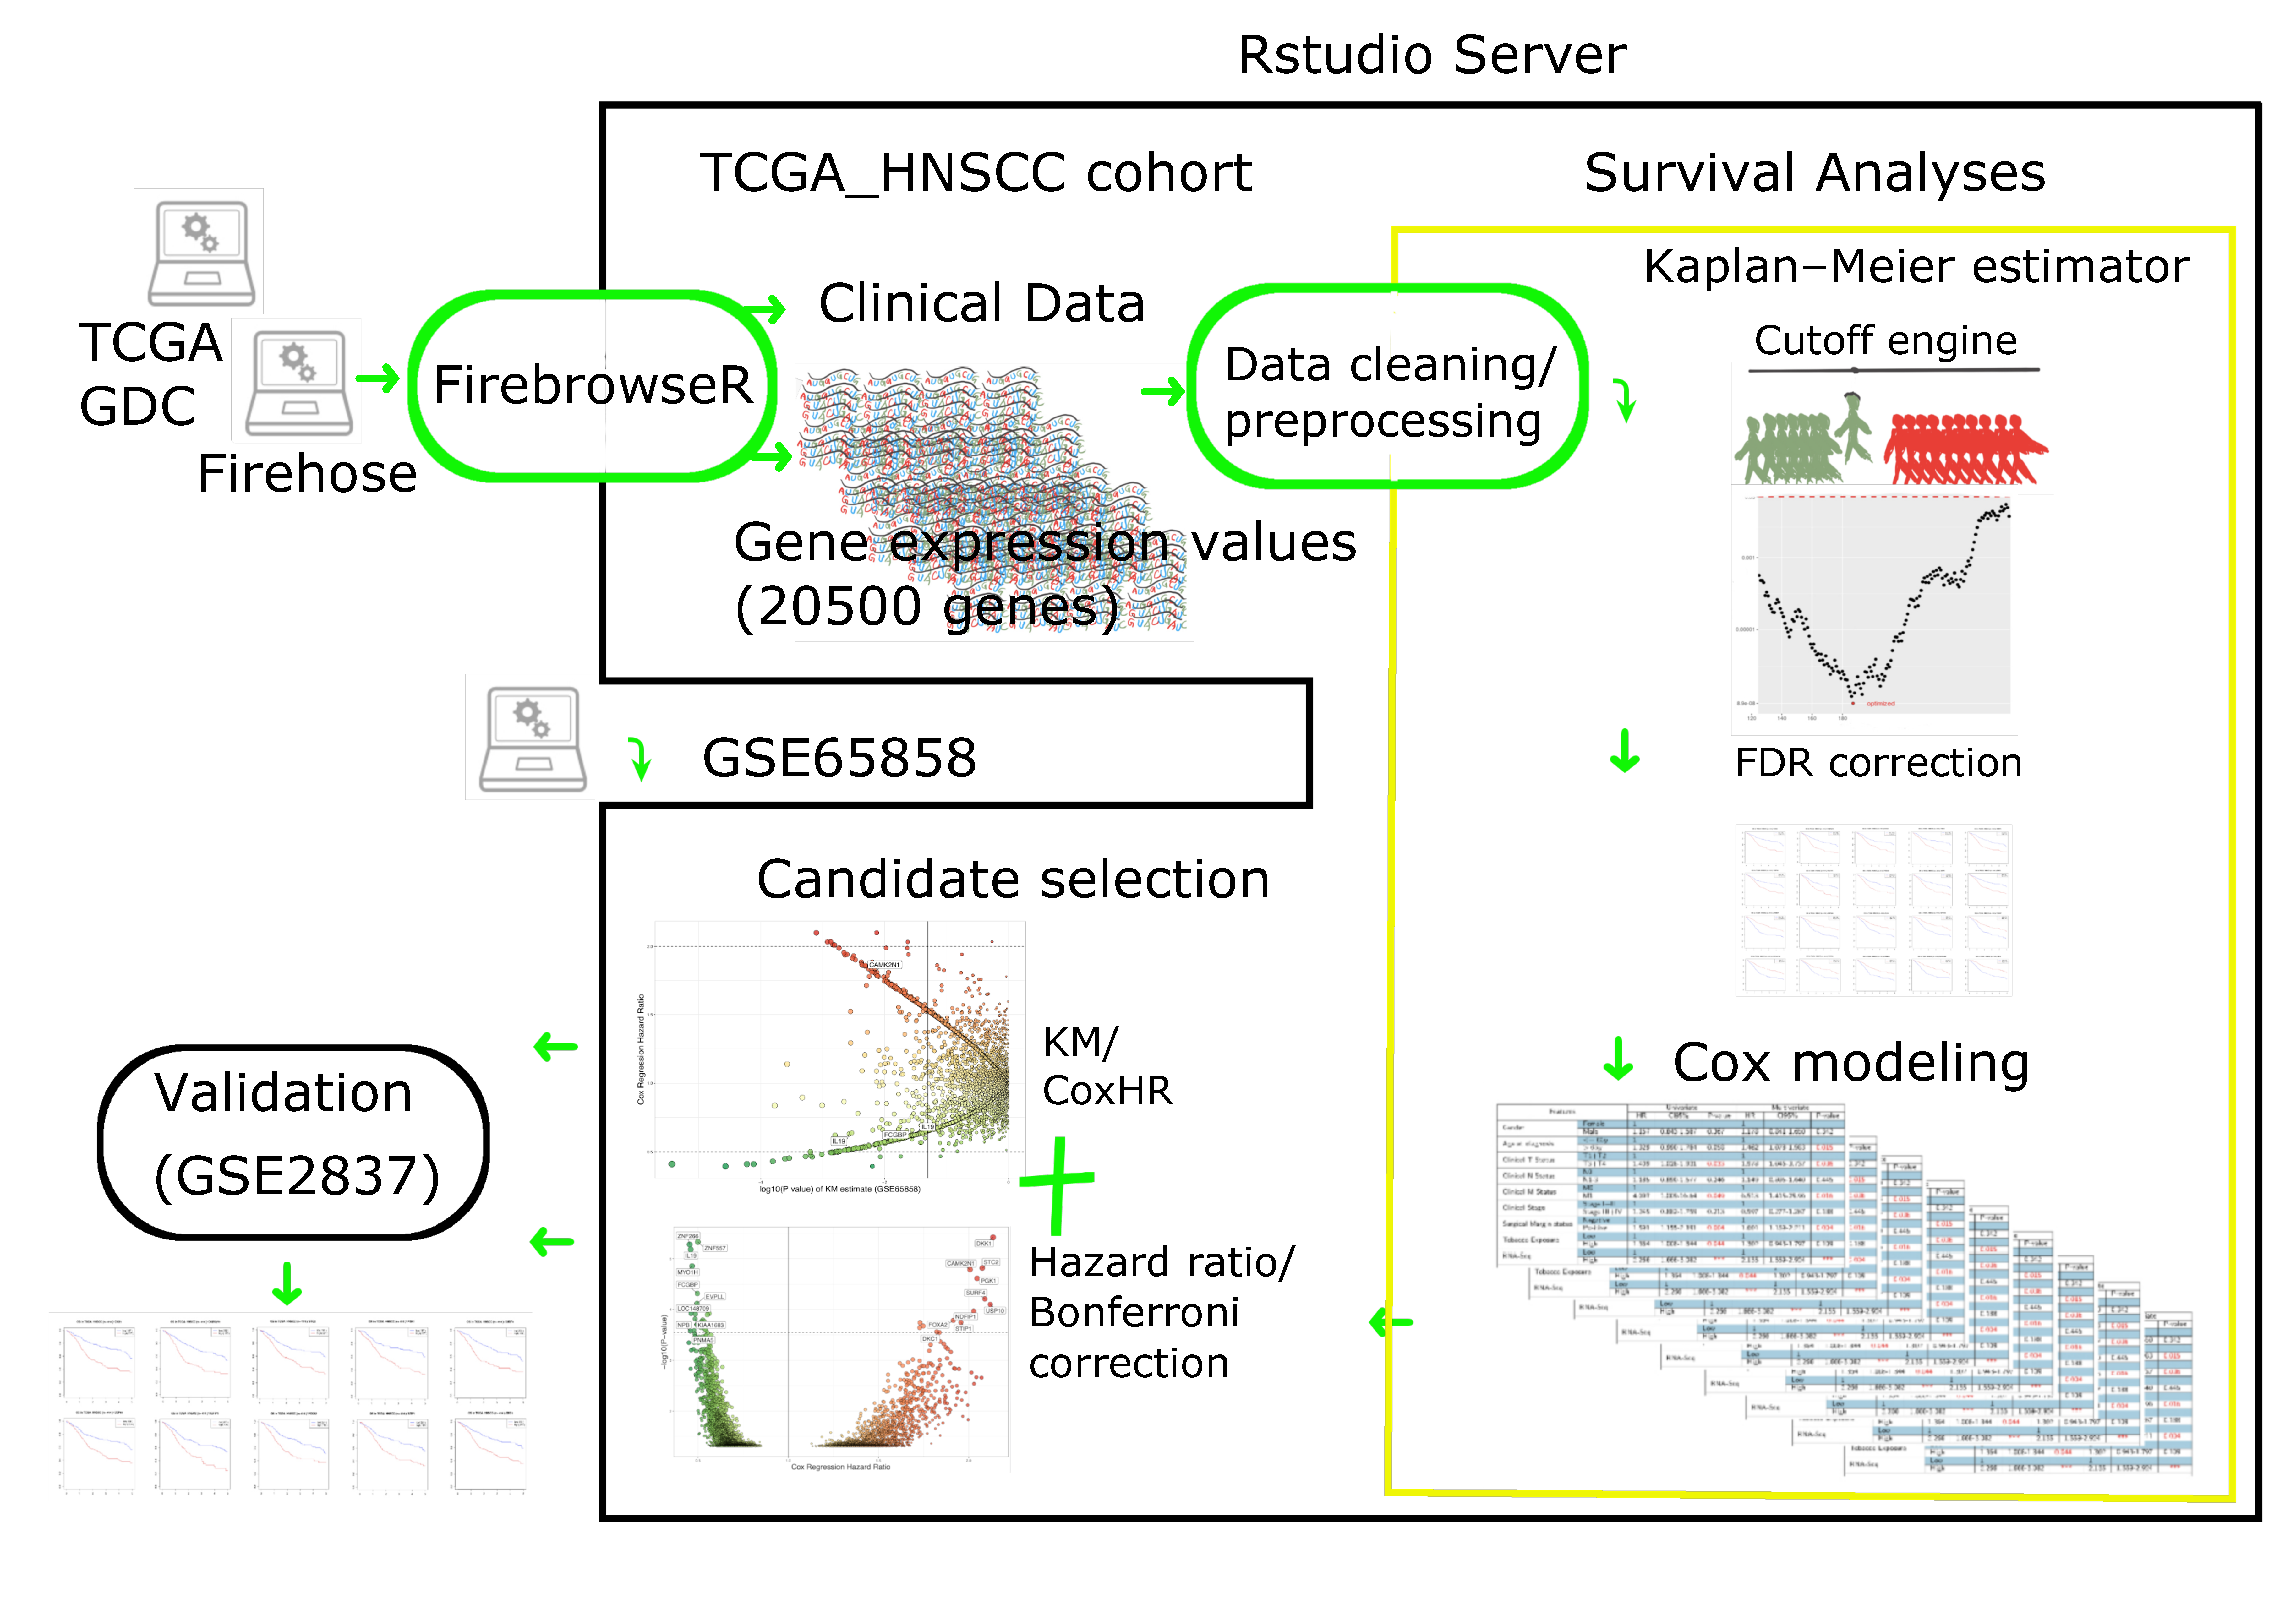
\includegraphics[width=14cm]{Figure_1_manuscript_workflow} % .PDF is better than .png
%, height=8cm
%\caption
\bcaption{A workflow of \acrshort{hnscc} biomarker discovery, step 1 (blue line: main procedure) and step 2 (orange line: analysis export).}
%Step 3 (purple line: dealing with surgical margin).
{The "main procedure" includes data retrieving from TCGA GDC data portal, data process with merging and cleaning, then performing the survival analyses. The Cutoff engine (cutofFinder\_func.HNSCC.R) might calculate all possible Kaplan-Meier P-value to find the optimal cutoff value of RNA-Seq for subsequent Cox modeling (a draft diagram shown on the upper right corner "HNSCC cohort", the serial cut for grouping patients with low [green] or high [red] expression of a specific gene, to yield a collection of P-values; please see Materials and Methods section for details). The step 2 "analysis export" performs dissecting and selection of candidate genes by Bonferroni adjusted P-value as well as a hazard ratio of Cox model, which was based on the results from the step 1.
(HNSCC: head and neck squamous cell carcinoma; TCGA: the Cancer Genome Atlas; RNA-Seq: RNA sequencing; GDC: Genomic Data Commons.)}
\label{fig:figure1}
\end{figure}

\clearpage
%%%%%%%%%%%%%%%%%%%%%%%%%%%%%%%%%%%%%%%%%%

\section{Results}


The 9416 Kaplan-Meier plots with associated Cox's univariate and multivariate tables were generated at workflow step 1 (see Figure \ref{fig:figure1}) and justified by the ranking of hazard ratios.
By uncorrected P-value below 0.05, we selected 967 genes in which \acrfull{hr} is greater than 1.5 or less than 0.5 (see Figure \ref{fig:figure2}(a) univariate, and Figure \ref{fig:figure2}(b)  multivariate plots). At the final step, a Bonferroni P-value correction was used to yield the twenty candidate genes, under the stringent criteria (see Figure \ref{fig:figure2}(c), (d)). The ten candidates, including DKK1, CAMK2N1, STC2, PGK1, SURF4, USP10, NDFIP1, FOXA2, STIP1, and DKC1, have significantly associated with the poor prognosis of \acrshort{os} (see Table \ref{table:table1}),
%\subsubsection{Figure 3}
while the other ten genes were over-expressed in the better survival patients, named as ZNF557, ZNF266, IL19, MYO1H, FCGBP, LOC148709, EVPLL, PNMA5, IQCN (previous name as KIAA1683), and NPB (see Table \ref{table:table3}, with their full name of genes).
We made a volcano plot for 9416 genes by Kaplan-Meier P-value (less than 0.05, obtained during cutoff finding procedure) against the Cox hazard ratio (see Figure \ref{fig:figure3}). The plot revealed that the most significant (Bonferroni-adjusted P-value $< 0.05$) candidate genes are located above the dotted line. At the same time, Cox's HR separated them on the two-side with prognostic impact.


%\subsubsection{Figure 2:h}
\begin{figure}[hp]
\centering
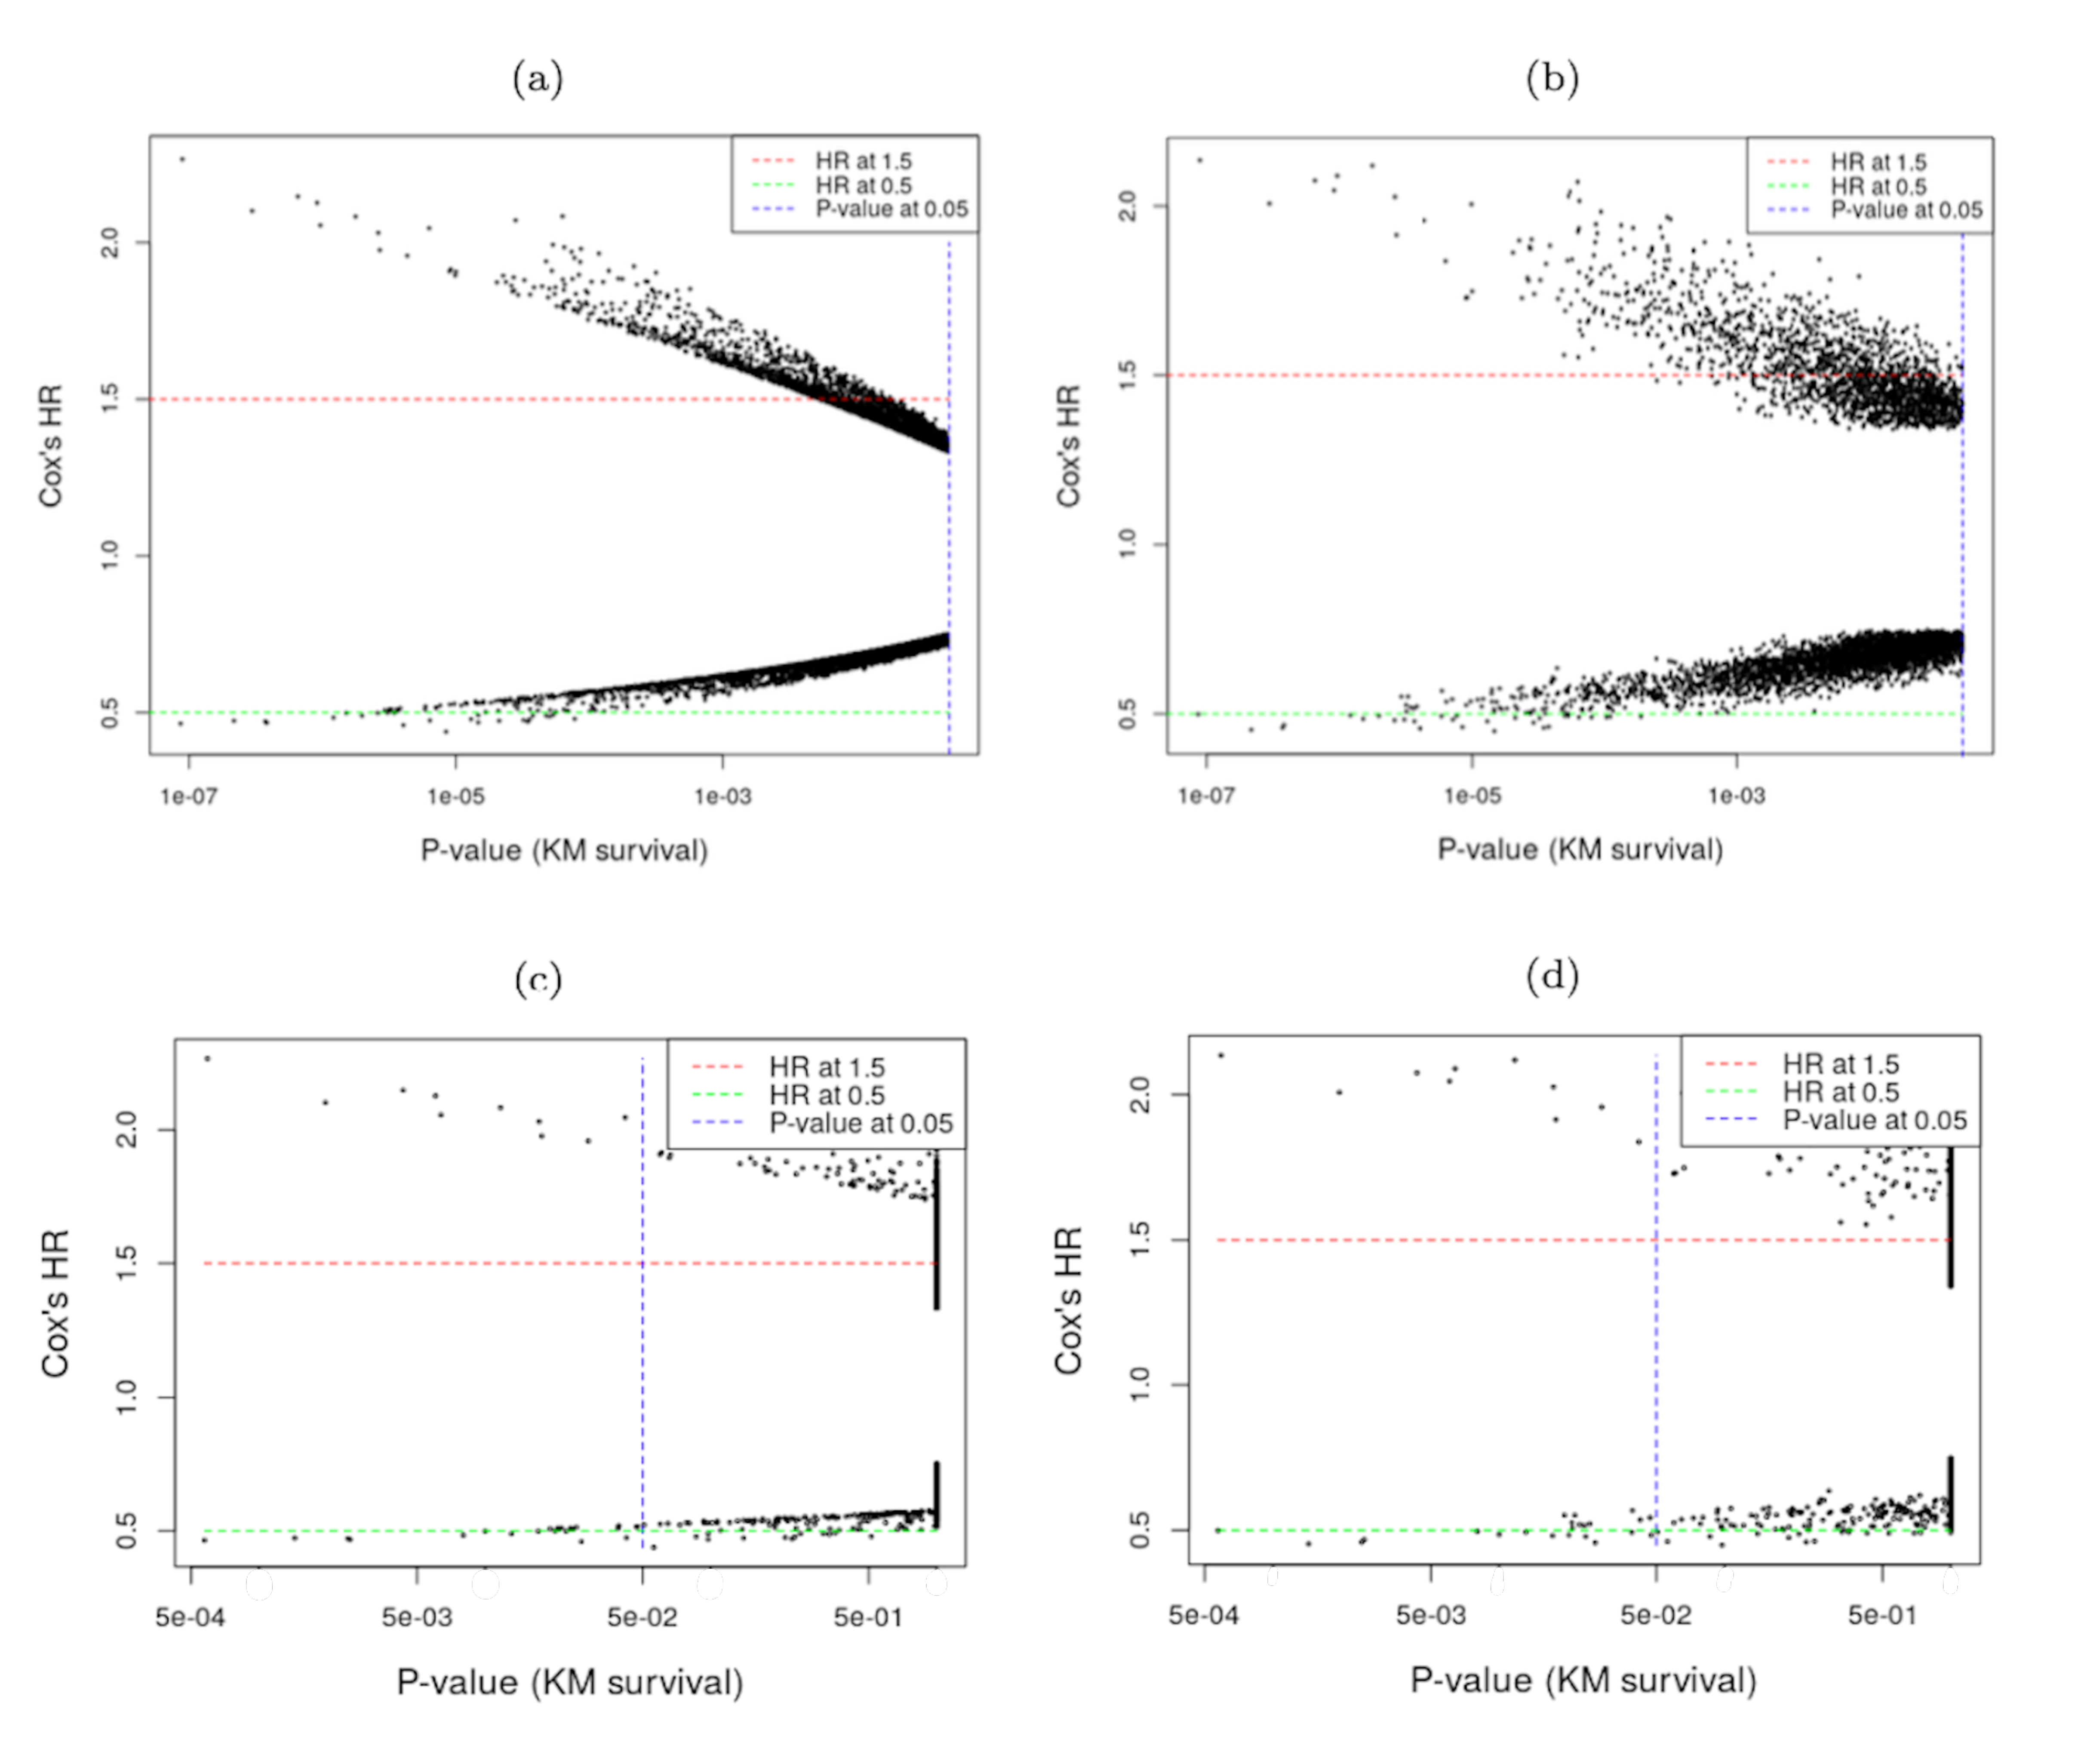
\includegraphics[width=14cm]{Figure2.pdf}
\bcaption{\acrshort{hnscc} Cox's hazard ratio and P-value plots.}
{(a) Univariate HR versus uncorrected P-value; (b) Multivariate HR versus uncorrected P-value; (c) Univariate HR versus Bonferroni corrected P-value; and (d) Multivariate HR versus Bonferroni corrected P-value.}
\label{fig:figure2}
\end{figure}

% tables 1  3
%%% tables
% Table1
% wide table \usepackage{tabularx}
% makecell{}

\begin{table}
%\begin{sidewaystable}[hp]
\centering
\caption{ The 10 candidate genes over-expressed with poor prognosis in \acrshort{hnscc} (ranked by Bonferroni adjusted P-value) }
\arrayrulecolor[rgb]{0.255,0.255,0.255}
\resizebox{\linewidth}{!}{
%\begin{tabular}{|l|l|l|l|l|l|l|l|c|}
\begin{tabularx}{\textwidth}{|l|p{3.5cm}|l|l|l|l|l|l|c|} % *** capital X or p{2cm}
% p{2cm}
\hline
\multicolumn{1}{|c|}{\multirow{2}{*}{Gene ID}} & \multicolumn{1}{c|}{\multirow{2}{*}{Gene Description}}     & \multicolumn{2}{c|}{Kaplan-Meier survival}                                                                                   & \multicolumn{2}{c|}{Univariate~}                                                        & \multicolumn{2}{c|}{Multivariate}                                                       & \multirow{2}{*}{Remark}                     \\ 
\cline{3-8}
\multicolumn{1}{|c|}{}                         & \multicolumn{1}{c|}{}                                      & \multicolumn{1}{c|}{P-value}               & \multicolumn{1}{c|}{\begin{tabular}[c]{@{}c@{}}Adjusted \\P-value\end{tabular}} & \multicolumn{1}{c|}{HR*}                   & 95\% CI                                    & HR*                                        & 95\% CI                                    &                                             \\ 
\hline
DKK1                                           & dickkopf WNT signaling pathway inhibitor 1                 & \num{8.9e-8}                               & 0.001                                                                           & 2.266                                      & 1.666-3.082                                & 2.135                                      & 1.559-2.924                                & **                                          \\ 
\hline
CAMK2N1                                        & calcium/calmodulin-dependent protein kinase II inhibitor 1 & \num{2.9e-7}                               & 0.002                                                                           & 2.101                                      & 1.572-2.809                                & 2.007                                      & 1.490-2.704                                & **                                          \\ 
\hline
STC2                                           & stanniocalcin 2                                            & \num{6.5e-7}                               & 0.004                                                                           & 2.147                                      & 1.578-2.921                                & 2.075                                      & 1.515-2.843                                & **                                          \\ 
\hline
PGK1                                           & phosphoglycerate kinase 1                                  & \num{9.1e-7}                               & 0.006                                                                           & 2.127                                      & 1.563-2.895                                & 2.046                                      & 1.498-2.795                                & **                                          \\ 
\hline
SURF4                                          & surfeit 4                                                  & \num{9.6e-7}                               & 0.006                                                                           & 2.055                                      & 1.531-2.757                                & 2.089                                      & 1.543-2.829                                & 3                                           \\ 
\hline
USP10                                          & ubiquitin specific peptidase 10                            & \num{1.7e-6}                               & 0.012                                                                           & 2.083                                      & 1.532-2.834                                & 2.119                                      & 1.551-2.895                                & **                                          \\ 
\hline
NDFIP1                                         & Nedd4 family interacting protein 1                         & \num{2.6e-6}                               & 0.017                                                                           & 2.031                                      & 1.502-2.746                                & 2.027                                      & 1.483-2.771                                & 6                                           \\ 
\hline
FOXA2                                          & forkhead box A2                                            & \num{2.7e-6}                               & 0.018                                                                           & 1.976                                      & 1.479-2.640                                & 1.914                                      & 1.426-2.569                                & **                                          \\ 
\hline
STIP1                                          & stress-induced-phosphoprotein 1                            & \num{4.3e-6}                              & 0.029                                                                           & 1.958                                      & 1.463-2.621                                & 1.957                                      & 1.451-2.640                                & **                                          \\ 
\hline
DKC1                                           & dyskeratosis congenita 1, dyskerin                         & \num{6.3e-6}                               & 0.042                                                                           & 2.046                                      & 1.490-2.808                                & 1.837                                      & 1.332-2.534                                & **                                          \\ 
\hline
\multicolumn{1}{|l!{\color{black}\vrule}}{}    & \multicolumn{1}{l!{\color{black}\vrule}}{}                 & \multicolumn{1}{l!{\color{black}\vrule}}{} & \multicolumn{1}{l!{\color{black}\vrule}}{}                                      & \multicolumn{1}{l!{\color{black}\vrule}}{} & \multicolumn{1}{l!{\color{black}\vrule}}{} & \multicolumn{1}{l!{\color{black}\vrule}}{} & \multicolumn{1}{l!{\color{black}\vrule}}{} & \multicolumn{1}{l!{\color{black}\vrule}}{}  \\ 
\arrayrulecolor{black}\hline
\multicolumn{9}{|l!{\color{black}\vrule}}{\begin{tabular}[c]{@{}l@{}}Selection criteria:~~\\~Kaplan-Meier Bonferroni adjusted P-value $< 0.05 $~\\~Cox's univariate and multivariate$ HR >= 1.5$ \end{tabular}}                                                                                                                                                                                                                                                              \\ 
\hline
\multicolumn{9}{|l!{\color{black}\vrule}}{* Cox's model: P-value $< 0.001$ }                                                                                                                                                                                                                                                                                                                                                                                                  \\ 
\hline
\multicolumn{9}{|l!{\color{black}\vrule}}{Remark: number of articles related with cancer research; ** as many~}                                                                                                                                                                                                                                                                                                                                                             \\
\hline
\end{tabularx}
}
\arrayrulecolor{black}
\label{table:table1}

%\end{sidewaystable}
\end{table}




%\subsubsection{Table3/legend}
%Table3. The 10 candidate genes over-expressed with better prognosis in HNSCC (ranked by Bonferroni corrected Kaplan-Meier P-value).
\begin{table}[hp]
\centering
\caption{The 10 candidate genes over-expressed with better prognosis in \acrshort{hnscc} (ranked by Bonferroni corrected P-value) }
\arrayrulecolor[rgb]{0.255,0.255,0.255}
\resizebox{\linewidth}{!}{%
\begin{tabular}{|l|l|l|l|l|l|l|l|c|} 
\hline
\multicolumn{1}{|c|}{\multirow{2}{*}{Gene ID}} & \multicolumn{1}{c|}{\multirow{2}{*}{Gene Description}} & \multicolumn{2}{l|}{Kaplan-Meier survival}                                                                                                                                                & \multicolumn{2}{c|}{Univariate~}                                                                        & \multicolumn{2}{c|}{Multivariate}                                                                       & \multicolumn{1}{l|}{\multirow{2}{*}{Remark}}  \\ 
\cline{3-8}
\multicolumn{1}{|c|}{}                         & \multicolumn{1}{c|}{}                                  & \multicolumn{1}{c!{\color{black}\vrule}}{P-value}                                  & \multicolumn{1}{c!{\color{black}\vrule}}{\begin{tabular}[c]{@{}c@{}}Adjusted\\~P-value\end{tabular}} & \multicolumn{1}{c!{\color{black}\vrule}}{HR*}   & \multicolumn{1}{c!{\color{black}\vrule}}{95\% CI}     & \multicolumn{1}{c!{\color{black}\vrule}}{HR*}   & \multicolumn{1}{c!{\color{black}\vrule}}{95\% CI}     & \multicolumn{1}{l|}{}                         \\ 
\cline{1-2}\arrayrulecolor{black}\cline{3-8}\arrayrulecolor[rgb]{0.255,0.255,0.255}\cline{9-9}
ZNF557                                         & zinc finger protein 557                                & \multicolumn{1}{l!{\color{black}\vrule}}{\textcolor[rgb]{0,0,0.471}{\num{8.6e-8}}} & \multicolumn{1}{l!{\color{black}\vrule}}{0.001}                                                      & \multicolumn{1}{l!{\color{black}\vrule}}{0.465} & \multicolumn{1}{l!{\color{black}\vrule}}{0.348-0.619} & \multicolumn{1}{l!{\color{black}\vrule}}{0.499} & \multicolumn{1}{l!{\color{black}\vrule}}{0.372-0.669} & 0                                             \\ 
\cline{1-2}\arrayrulecolor{black}\cline{3-8}\arrayrulecolor[rgb]{0.255,0.255,0.255}\cline{9-9}
ZNF266                                         & zinc finger protein 266                                & \textcolor[rgb]{0,0,0.471}{\num{2.2e-7}}                                           & 0.001                                                                                                & 0.474                                           & 0.355-0.632                                           & 0.453                                           & 0.338-0.607                                           & 1                                             \\ 
\hline
IL19                                           & interleukin 19                                         & \textcolor[rgb]{0,0,0.471}{}\num{3.7e-7}\textcolor[rgb]{0,0,0.471}{}               & 0.002                                                                                                & 0.472                                           & 0.351-0.635                                           & 0.459                                           & 0.340-0.619                                           & 14                                            \\ 
\hline
MYO1H                                          & myosin 1H                                              & \textcolor[rgb]{0,0,0.471}{}\num{3.8e-7}\textcolor[rgb]{0,0,0.471}{}               & 0.003                                                                                                & 0.468                                           & 0.347-0.632                                           & 0.467                                           & 0.344-0.634                                           & 0                                             \\ 
\hline
FCGBP                                          & Fc fragment of IgG binding protein                     & \textcolor[rgb]{0,0,0.471}{}\num{1.2e-6}\textcolor[rgb]{0,0,0.471}{}               & 0.008                                                                                                & 0.484                                           & 0.359-0.653                                           & 0.496                                           & 0.366-0.674                                           & **                                            \\ 
\hline
LOC148709                                      & LncRNA LOC148709                                       & \textcolor[rgb]{0,0,0.471}{\num{1.5e-6}}                                           & 0.010                                                                                                & 0.499                                           & 0.374-0.666                                           & 0.485                                           & 0.361-0.652                                           & 1                                             \\ 
\hline
EVPLL                                          & envoplakin-like protein                                & \textcolor[rgb]{0,0,0.471}{\num{2.0e-6}}                                           & 0.013                                                                                                & 0.490                                           & 0.363-0.661                                           & 0.494                                           & 0.364-0.672                                           & 0                                             \\ 
\hline
PNMA5                                          & paraneoplastic antigen like 5                          & \textcolor[rgb]{0,0,0.471}{\num{2.6e-6}}                                           & 0.017                                                                                                & 0.499                                           & 0.371-0.671                                           & 0.481                                           & 0.357-0.650                                           & 5                                             \\ 
\hline
KIAA1683                                       & new name as IQ Motif Containing N (IQCN)                           & \textcolor[rgb]{0,0,0.471}{\num{3.1e-6}}                                           & 0.020                                                                                                & 0.500                                           & 0.371-0.673                                           & 0.483                                           & 0.356-0.654                                           & 0                                             \\ 
\hline
NPB                                            & neuropeptide B                                         & \textcolor[rgb]{0,0,0.471}{\num{4.0e-6}}                                           & 0.027                                                                                                & 0.460                                           & 0.328-0.646                                           & 0.457                                           & 0.324-0.646                                           & 4                                             \\ 
\hline
                                               &                                                        &                                                                                    &                                                                                                      &                                                 &                                                       &                                                 &                                                       & \multicolumn{1}{l|}{}                         \\ 
\hline
\multicolumn{9}{|l|}{\begin{tabular}[c]{@{}l@{}}Selection criteria:~\\~Kaplan-Meier Bonferroni adjusted P-value \textless{} 0.05~\\~Cox's univariate and multivariate HR \textgreater{}= 1.5\\* Cox's model: P-value \textless{} 0.001\\Remark: number off articles related to cancer research; ** as many~\\lncRNA: Long non-coding RNA\end{tabular}}                                                                                                                                                                                                                 \\
\hline
\end{tabular}
}
\arrayrulecolor{black}
\label{table:table3}
\end{table}




%\subsubsection{Figure 3:h}
\begin{figure}[hp]
\centering
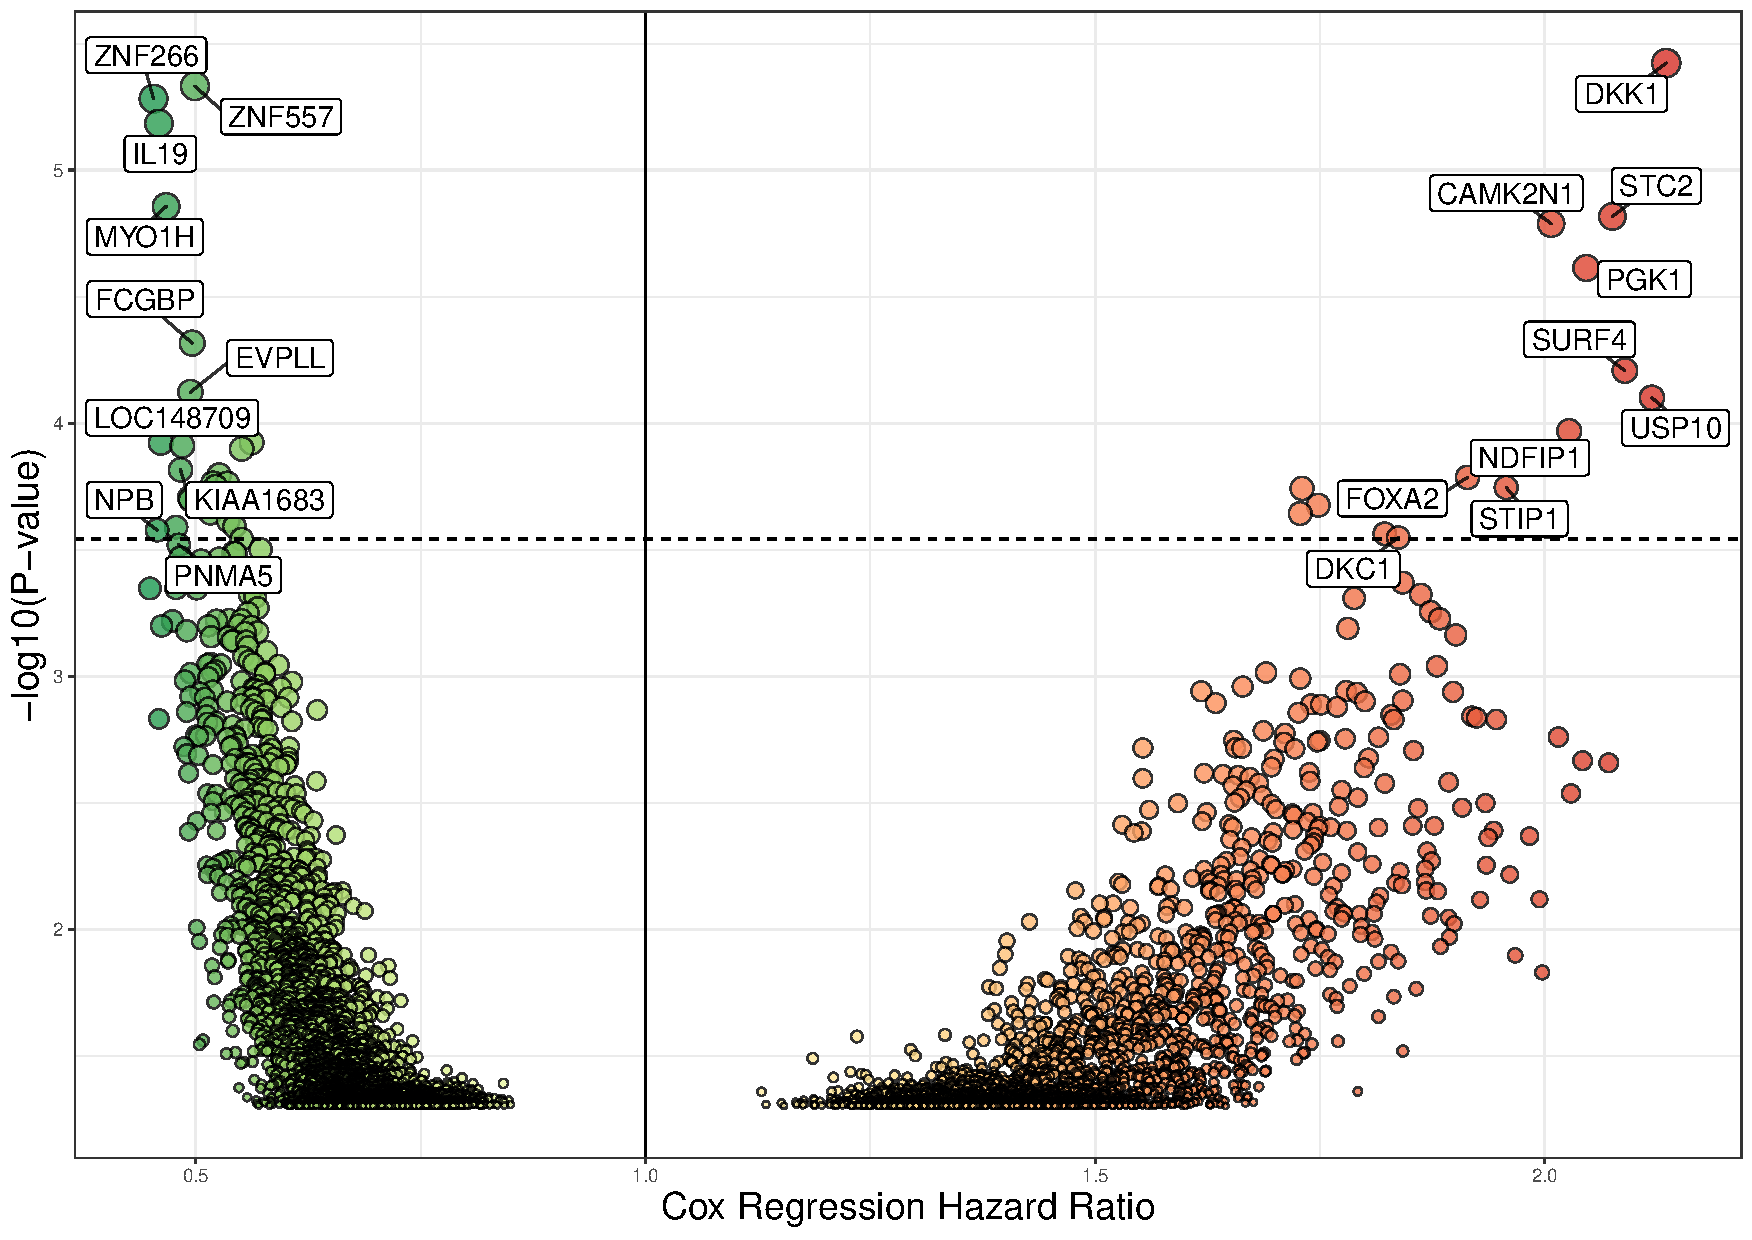
\includegraphics[width=14cm]{TCGA_HNSC_Optimal_Overall_allPlot_unKM_P_multiHR-Figure3.pdf} % .png from PvalueplotKM_20genes_Bonf.pdf
\bcaption{Volcano plot of genes under survival analyses.}
{X axis: unadjusted P-value of Kaplan-Meier survival (-log10 transformed).
Y axis: multivariate hazard ratio from Cox proportional regression model.
Dotted line: significant Bonferroni corrected P-value. 
Red circles mark 10 candidate genes, which impact on poor prognosis ($HR>=1.5$). Green circles mark 10 genes, which affect on better survival ($HR<=0.5$).}
\label{fig:figure3}
\end{figure}
% new figure of volcano plot: TCGA_HNSC_Optimal_Overall_allPlot_unKM_P_multiHR.pdf, -log10(raw KM P-value) vs Cox multivariate HR
% X axis: "frequency" (number of uncorrected P-values less than 0.05 during Kaplan-Meier cutoff finding procedure). X axis: adjusted Kaplan-Meier P-value.

\clearpage


Our top 1 candidate is \acrfull{DKK1} (see Figure \ref{fig:figure4}(a)). The Kaplan-Meier curve revealed 227 patients bearing the higher expression of \acrshort{DKK1} were suffered from only 40\% of 5-year \acrshort{os} rate. In comparison, the other 187 patients with lower expression (the cutoff at -0.312(RSEM)) have been a better prognosis (adjusted P-value as $0.001$).
Figure \ref{fig:figure4}(b)'s cumulative P-value plot showed that the uncorrected 116 P-values ($< 0.05$) were estimated by a serial cut from 125 to 290 persons for grouping the cohort in our cutoff finding procedure (cutofFinder\_func.R, see Figure \ref{fig:figure1}, "HNSCC cohort"). The smallest P-value (\num{8.9e-8}), when cut on n=187 (45.2\% of 414), was defined as optimal P-value.
Conversely, the most associated gene with better survival is \acrfull{ZNF557}. In Figure \ref{fig:figure4}(c), a Kaplan-Meier curve revealed 264 patients bearing the higher expression of \acrshort{ZNF557} have 55\% of 5-year OS survival rate (adjusted P-value = $0.001$). The cutoff finding procedure (cutofFinder\_func.R) generated cumulative P-value plots in Figure \ref{fig:figure4}(d). There were 166 uncorrected P-values estimated by a serial cut from 125 to 290 for grouping the cohort. All was less than 0.05, and the smallest P-value (\num{8.6e-8}), when cut on n=150 (36.2\% of total cohort 414), was defined as optimal P-value with a cutoff value -0.511(RSEM) of \acrshort{rnaseq}.
%The second candidate, which improving patient survival, is ZNF266.
%\subsubsection{Tables} in main article

%\subsubsection{Figure 4:h}
\begin{figure}[hp]
\centering
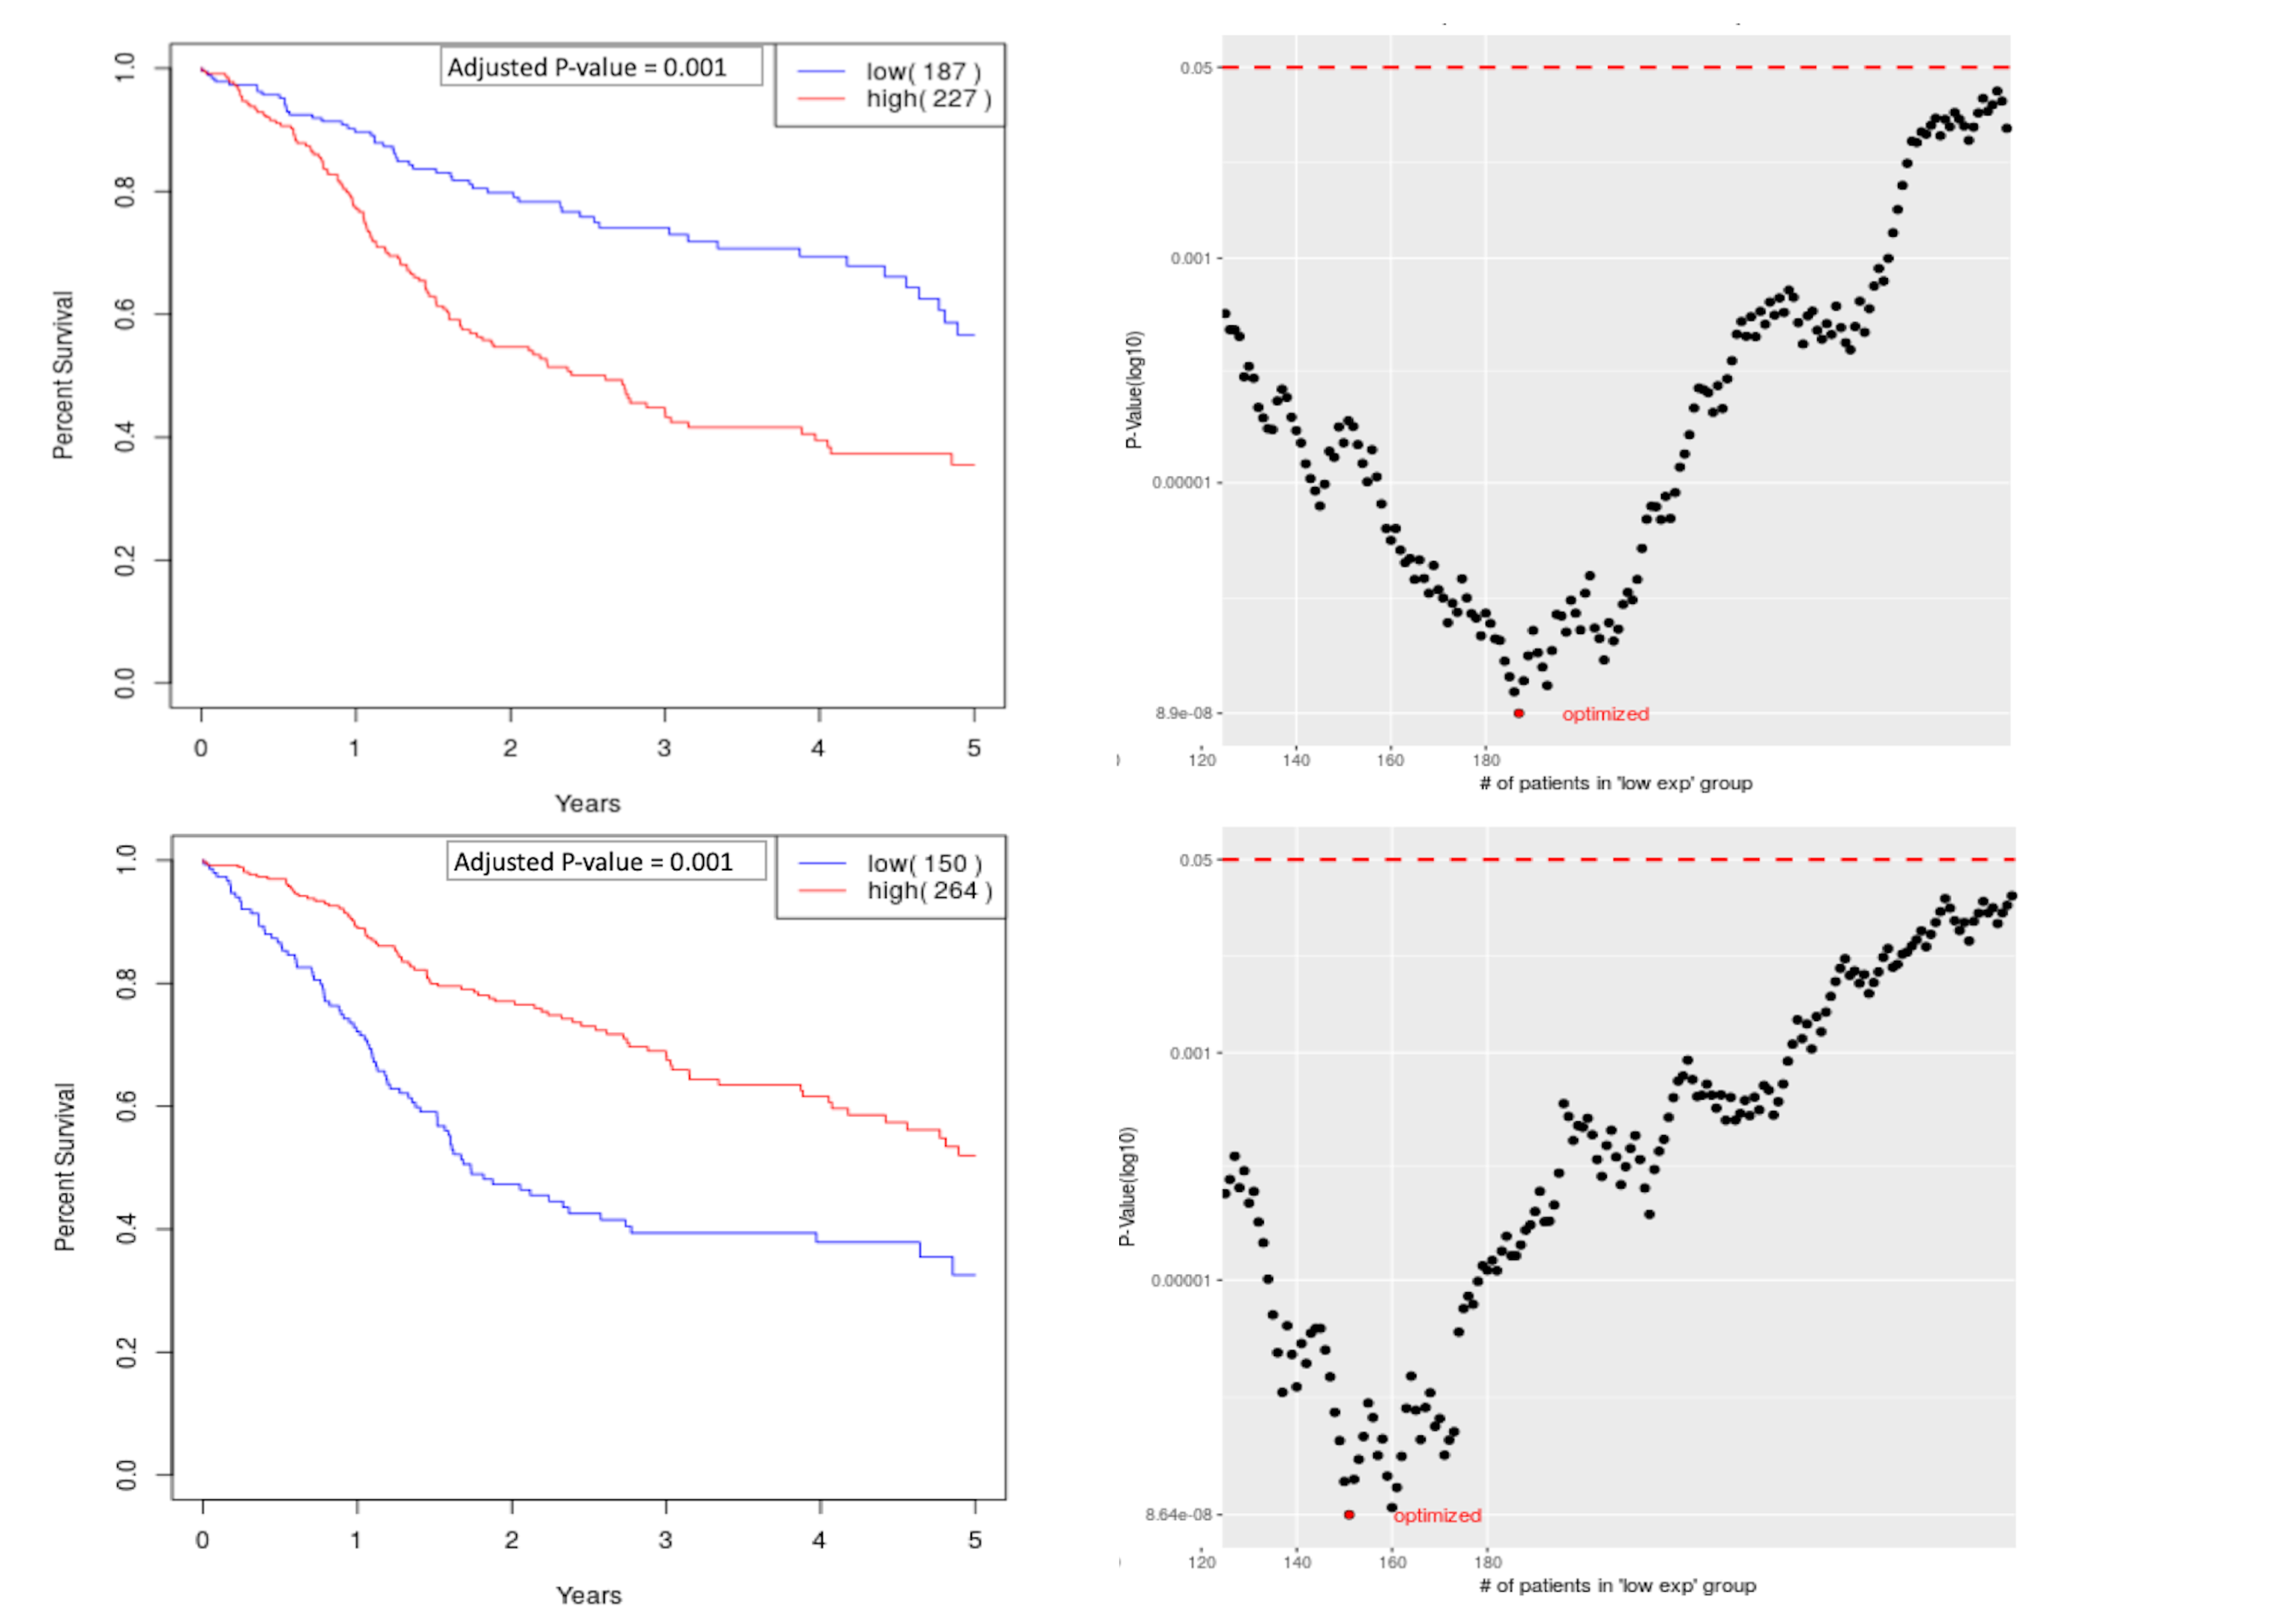
\includegraphics[width=15cm]{Figure4.pdf}
\bcaption{Kaplan-Meier survival analyses, by cutoff finding.}
{(a) Kaplan-Meier plot of DKK1 under optimal P-value, and (b) the cutoff was derived from cumulative P-value plots of DKK1. (c) Kaplan-Meier plot of ZNF557 under optimal P-value, and (d) the cutoff was derived from cumulative P-value plots of ZNF557.}
\label{fig:figure4}
\end{figure}

\clearpage

Table \ref{table:table1} showed ten candidate genes over-expressed with poor prognosis in \acrshort{hnscc}, ranked by adjusted Kaplan-Meier P-value. We found their Cox's univariate and multivariate HR are all greater than 1.837. There were few published articles of \acrfull{SURF4} and \acrfull{NDFIP1} (\acrshort{NEDD4}: \acrlong{NEDD4}), which were related to cancer research.
In Table \ref{table:table2},
after adjustment of confounders, it was considered the \acrshort{DKK1} over-expression is the independent prognostic factor (multivariate HR 2.135 [95\% CI: 1.559-2.924, P-value $<$ 0.001]), as well as clinical T stage (HR 1.978 [95\% CI: 1.046-3.737, P-value = 0.036]) and surgical margins status (HR 1.601 [95\% CI: 1.159-2.211, P-value = 0.004]). The age older than 65 year-old has negative influence on survival (HR 1.462 [95\% CI: 1.078-1.983, P-value = 0.015]). The M stage could not be considered due to only 3 out of 414 patients which have distant metastasis.

%\subsubsection{Table2/legend}
%Table 2. Univariate/Multivariate Cox's proportional hazards regression analyses on OS time of DKK1 gene expression in HNSCC.
%(P-value Significant codes is denoted as  0.01 mark as *; 0.001 mark as **; if $<$0.001  mark as ***)
\begin{table}[hp]
\centering
\caption{Univariate/multivariate Cox's proportional hazards regression analyses on OS time of DKK1 gene expression in \acrshort{hnscc}}
\arrayrulecolor[rgb]{0.255,0.255,0.255}
\resizebox{\linewidth}{!}{%
\begin{tabular}{|l|l|l|l|l|l|l|l|} 
\arrayrulecolor{black}\cline{1-2}\arrayrulecolor[rgb]{0.255,0.255,0.255}\cline{3-8}
\multicolumn{2}{|c!{\color{black}\vrule}}{\multirow{2}{*}{Features}}                                                          & \multicolumn{3}{c|}{Univariate}                                                                                                                                                                                                                & \multicolumn{3}{c|}{Multivariate}                                                                                                                                                                                                               \\ 
\cline{3-8}
\multicolumn{2}{|c!{\color{black}\vrule}}{}                                                                                   & \multicolumn{1}{c!{\color{black}\vrule}}{HR}                                   & \multicolumn{1}{c!{\color{black}\vrule}}{CI95\%}                              & \multicolumn{1}{c!{\color{black}\vrule}}{P-value}                             & \multicolumn{1}{c!{\color{black}\vrule}}{HR}                                   & \multicolumn{1}{c!{\color{black}\vrule}}{CI95\%}                              & \multicolumn{1}{c!{\color{black}\vrule}}{P-value}                              \\ 
\arrayrulecolor{black}\hline
\multirow{2}{*}{Gender}                 & \multicolumn{1}{l!{\color{black}\vrule}}{{\cellcolor[rgb]{0.62,0.812,0.878}}Female} & \multicolumn{1}{l!{\color{black}\vrule}}{{\cellcolor[rgb]{0.62,0.812,0.878}}1} & \multicolumn{1}{l!{\color{black}\vrule}}{{\cellcolor[rgb]{0.62,0.812,0.878}}} & \multicolumn{1}{l!{\color{black}\vrule}}{{\cellcolor[rgb]{0.62,0.812,0.878}}} & \multicolumn{1}{l!{\color{black}\vrule}}{{\cellcolor[rgb]{0.62,0.812,0.878}}1} & \multicolumn{1}{l!{\color{black}\vrule}}{{\cellcolor[rgb]{0.62,0.812,0.878}}} & \multicolumn{1}{l!{\color{black}\vrule}}{{\cellcolor[rgb]{0.62,0.812,0.878}}}  \\ 
\cline{2-8}
                                        & Male                                                                                & 1.157                                                                          & 0.843-1.587                                                                   & 0.367                                                                         & 1.178                                                                          & 0.841-1.650                                                                   & 0.342                                                                          \\ 
\arrayrulecolor[rgb]{0.255,0.255,0.255}\hline
\multirow{2}{*}{Age at diagnosis}       & {\cellcolor[rgb]{0.62,0.812,0.878}}$<=65y$                                          & {\cellcolor[rgb]{0.62,0.812,0.878}}1                                           & {\cellcolor[rgb]{0.62,0.812,0.878}}                                           & {\cellcolor[rgb]{0.62,0.812,0.878}}                                           & {\cellcolor[rgb]{0.62,0.812,0.878}}1                                           & {\cellcolor[rgb]{0.62,0.812,0.878}}                                           & {\cellcolor[rgb]{0.62,0.812,0.878}}                                            \\ 
\cline{2-8}
                                        & $>65y$                                                                              & 1.329                                                                          & 0.990-1.784                                                                   & 0.058                                                                         & 1.462                                                                          & 1.078-1.983                                                                   & \textcolor{red}{0.015}                                                         \\ 
\hline
\multirow{2}{*}{Clinical T Status}      & {\cellcolor[rgb]{0.62,0.812,0.878}}T1+T2                                            & {\cellcolor[rgb]{0.62,0.812,0.878}}1                                           & {\cellcolor[rgb]{0.62,0.812,0.878}}                                           & {\cellcolor[rgb]{0.62,0.812,0.878}}                                           & {\cellcolor[rgb]{0.62,0.812,0.878}}1                                           & {\cellcolor[rgb]{0.62,0.812,0.878}}                                           & {\cellcolor[rgb]{0.62,0.812,0.878}}                                            \\ 
\cline{2-8}
                                        & T3+T4                                                                               & 1.409                                                                          & 1.028-1.931                                                                   & \textcolor{red}{0.033}                                                        & 1.978                                                                          & 1.046-3.737                                                                   & \textcolor{red}{0.036}                                                         \\ 
\hline
\multirow{2}{*}{Clinical N Status}      & {\cellcolor[rgb]{0.62,0.812,0.878}}N0                                               & {\cellcolor[rgb]{0.62,0.812,0.878}}1                                           & {\cellcolor[rgb]{0.62,0.812,0.878}}                                           & {\cellcolor[rgb]{0.62,0.812,0.878}}                                           & {\cellcolor[rgb]{0.62,0.812,0.878}}1                                           & {\cellcolor[rgb]{0.62,0.812,0.878}}                                           & {\cellcolor[rgb]{0.62,0.812,0.878}}                                            \\ 
\cline{2-8}
                                        & N1-3                                                                                & 1.185                                                                          & 0.890-1.577                                                                   & 0.246                                                                         & 1.149                                                                          & 0.805-1.640                                                                   & 0.445                                                                          \\ 
\hline
\multirow{2}{*}{Clinical M Status}      & {\cellcolor[rgb]{0.62,0.812,0.878}}M0                                               & {\cellcolor[rgb]{0.62,0.812,0.878}}1                                           & {\cellcolor[rgb]{0.62,0.812,0.878}}                                           & {\cellcolor[rgb]{0.62,0.812,0.878}}                                           & {\cellcolor[rgb]{0.62,0.812,0.878}}1                                           & {\cellcolor[rgb]{0.62,0.812,0.878}}                                           & {\cellcolor[rgb]{0.62,0.812,0.878}}                                            \\ 
\cline{2-8}
                                        & M1                                                                                  & 4.097                                                                          & 1.009-16.64                                                                   & \textcolor{red}{0.049}                                                        & 6.513                                                                          & 1.415-29.96                                                                   & \textcolor{red}{0.016}                                                         \\ 
\hline
\multirow{2}{*}{Clinical Stage}         & {\cellcolor[rgb]{0.62,0.812,0.878}}Stage I+II                                       & {\cellcolor[rgb]{0.62,0.812,0.878}}1                                           & {\cellcolor[rgb]{0.62,0.812,0.878}}                                           & {\cellcolor[rgb]{0.62,0.812,0.878}}                                           & {\cellcolor[rgb]{0.62,0.812,0.878}}1                                           & {\cellcolor[rgb]{0.62,0.812,0.878}}                                           & {\cellcolor[rgb]{0.62,0.812,0.878}}                                            \\ 
\cline{2-8}
                                        & Stage III+IV                                                                        & 1.245                                                                          & 0.882-1.759                                                                   & 0.213                                                                         & 0.597                                                                          & 0.277-1.287                                                                   & 0.188                                                                          \\ 
\hline
\multirow{2}{*}{Surgical Margin status} & {\cellcolor[rgb]{0.62,0.812,0.878}}Negative                                         & {\cellcolor[rgb]{0.62,0.812,0.878}}1                                           & {\cellcolor[rgb]{0.62,0.812,0.878}}                                           & {\cellcolor[rgb]{0.62,0.812,0.878}}                                           & {\cellcolor[rgb]{0.62,0.812,0.878}}1                                           & {\cellcolor[rgb]{0.62,0.812,0.878}}                                           & {\cellcolor[rgb]{0.62,0.812,0.878}}                                            \\ 
\cline{2-8}
                                        & Positive                                                                            & 1.591                                                                          & 1.155-2.191                                                                   & \textcolor{red}{0.004}                                                        & 1.601                                                                          & 1.159-2.211                                                                   & \textcolor{red}{0.004}                                                         \\ 
\hline
\multirow{2}{*}{Tobacco Exposure}       & {\cellcolor[rgb]{0.62,0.812,0.878}}Low                                              & {\cellcolor[rgb]{0.62,0.812,0.878}}1                                           & {\cellcolor[rgb]{0.62,0.812,0.878}}                                           & {\cellcolor[rgb]{0.62,0.812,0.878}}                                           & {\cellcolor[rgb]{0.62,0.812,0.878}}1                                           & {\cellcolor[rgb]{0.62,0.812,0.878}}                                           & {\cellcolor[rgb]{0.62,0.812,0.878}}                                            \\ 
\cline{2-8}
                                        & High                                                                                & 1.364                                                                          & 1.008-1.844                                                                   & \textcolor{red}{0.044}                                                        & 1.302                                                                          & 0.943-1.797                                                                   & 0.109                                                                          \\ 
\hline
\multirow{2}{*}{RNA-Seq}                & {\cellcolor[rgb]{0.62,0.812,0.878}}Low                                              & {\cellcolor[rgb]{0.62,0.812,0.878}}1                                           & {\cellcolor[rgb]{0.62,0.812,0.878}}                                           & {\cellcolor[rgb]{0.62,0.812,0.878}}                                           & {\cellcolor[rgb]{0.62,0.812,0.878}}1                                           & {\cellcolor[rgb]{0.62,0.812,0.878}}                                           & {\cellcolor[rgb]{0.62,0.812,0.878}}                                            \\ 
\cline{2-8}
                                        & High                                                                                & 2.266                                                                          & 1.666-3.082                                                                   & \multicolumn{1}{c|}{\textcolor{red}{***}}                                     & 2.135                                                                          & 1.559-2.924                                                                   & \multicolumn{1}{c|}{\textcolor{red}{***}}                                      \\ 
\hline
\multicolumn{8}{|l|}{}                                                                                                                                                                                                                                                                                                                                                                                                                                                                                                                                                                                                           \\ 
\hline
\multicolumn{8}{|l|}{(P-value significant codes is denoted: $red<0.05$; *** $<0.001$~~)}                                                                                                                                                                                                                                                                                                                                                                                                                                                                                                                                           \\
\hline
\end{tabular}
}
\arrayrulecolor{black}
\label{table:table2}
\end{table}




There were also ten candidate genes over-expressed with a better prognosis of \acrshort{hnscc}, listed in Table \ref{table:table3}. Cox's univariate and multivariate HR is just under 0.5.
In Table \ref{table:table4},
after adjustment of confounders, it revealed HR 1.961 [95\% CI: 1.035-3.714, P-value = 0.039] in advance clinical T Status, HR 1.631 [95\% CI: 1.18-2.254, P-value = 0.003] with positive surgical margin involvement, HR 1.453 [95\% CI: 1.055-2.000, P-value = 0.022] with higher tobacco exposure, and a protective HR 0.499 [95\% CI: 0.372-0.669, P-value $<$ 0.001] in over-expressed \acrshort{ZNF557} gene.

In overall results, those 20 candidate biomarkers, clinical T stage, and surgical margin are independent prognosis factors in \acrshort{hnscc}.



%\subsubsection{Table4/legend}
\begin{table}[!hp]
\centering
\caption{Univariate/multivariate Cox's proportional hazards regression analyses on OS time of ZNF557 gene expression in \acrshort{hnscc}}
\arrayrulecolor[rgb]{0.255,0.255,0.255}
\resizebox{\linewidth}{!}{%
\begin{tabular}{|l|l|l|l|l|l|l|l|} 
\arrayrulecolor{black}\cline{1-2}\arrayrulecolor[rgb]{0.255,0.255,0.255}\cline{3-8}
\multicolumn{2}{|c!{\color{black}\vrule}}{\multirow{2}{*}{Features}}                                                          & \multicolumn{3}{c|}{Univariate}                                                                                                                                                                                                                & \multicolumn{3}{c|}{Multivariate}                                                                                                                                                                                                               \\ 
\cline{3-8}
\multicolumn{2}{|c!{\color{black}\vrule}}{}                                                                                   & \multicolumn{1}{c!{\color{black}\vrule}}{HR}                                   & \multicolumn{1}{c!{\color{black}\vrule}}{CI95\%}                              & \multicolumn{1}{c!{\color{black}\vrule}}{P-value}                             & \multicolumn{1}{c!{\color{black}\vrule}}{HR}                                   & \multicolumn{1}{c!{\color{black}\vrule}}{CI95\%}                              & \multicolumn{1}{c!{\color{black}\vrule}}{P-value}                              \\ 
\arrayrulecolor{black}\hline
\multirow{2}{*}{Gender}                 & \multicolumn{1}{l!{\color{black}\vrule}}{{\cellcolor[rgb]{0.62,0.812,0.878}}Female} & \multicolumn{1}{l!{\color{black}\vrule}}{{\cellcolor[rgb]{0.62,0.812,0.878}}1} & \multicolumn{1}{l!{\color{black}\vrule}}{{\cellcolor[rgb]{0.62,0.812,0.878}}} & \multicolumn{1}{l!{\color{black}\vrule}}{{\cellcolor[rgb]{0.62,0.812,0.878}}} & \multicolumn{1}{l!{\color{black}\vrule}}{{\cellcolor[rgb]{0.62,0.812,0.878}}1} & \multicolumn{1}{l!{\color{black}\vrule}}{{\cellcolor[rgb]{0.62,0.812,0.878}}} & \multicolumn{1}{l!{\color{black}\vrule}}{{\cellcolor[rgb]{0.62,0.812,0.878}}}  \\ 
\cline{2-8}
                                        & Male                                                                                & 1.157                                                                          & 0.843-1.587                                                                   & 0.367                                                                         & 1.163                                                                          & 0.833-1.625                                                                   & 0.375                                                                          \\ 
\arrayrulecolor[rgb]{0.255,0.255,0.255}\hline
\multirow{2}{*}{Age at diagnosis}       & {\cellcolor[rgb]{0.62,0.812,0.878}}$<=65y$                                          & {\cellcolor[rgb]{0.62,0.812,0.878}}1                                           & {\cellcolor[rgb]{0.62,0.812,0.878}}                                           & {\cellcolor[rgb]{0.62,0.812,0.878}}                                           & {\cellcolor[rgb]{0.62,0.812,0.878}}1                                           & {\cellcolor[rgb]{0.62,0.812,0.878}}                                           & {\cellcolor[rgb]{0.62,0.812,0.878}}                                            \\ 
\cline{2-8}
                                        & $>65y$                                                                              & 1.329                                                                          & 0.990-1.784                                                                   & 0.058                                                                         & 1.328                                                                          & 0.976-1.808                                                                   & 0.071                                                                          \\ 
\hline
\multirow{2}{*}{Clinical T Status}      & {\cellcolor[rgb]{0.62,0.812,0.878}}T1+T2                                            & {\cellcolor[rgb]{0.62,0.812,0.878}}1                                           & {\cellcolor[rgb]{0.62,0.812,0.878}}                                           & {\cellcolor[rgb]{0.62,0.812,0.878}}                                           & {\cellcolor[rgb]{0.62,0.812,0.878}}1                                           & {\cellcolor[rgb]{0.62,0.812,0.878}}                                           & {\cellcolor[rgb]{0.62,0.812,0.878}}                                            \\ 
\cline{2-8}
                                        & T3+T4                                                                               & 1.409                                                                          & 1.028-1.931                                                                   & \textcolor[rgb]{1,0.149,0}{0.033}                                             & 1.961                                                                          & 1.035-3.714                                                                   & \textcolor[rgb]{1,0.149,0}{0.039}                                              \\ 
\hline
\multirow{2}{*}{Clinical N Status}      & {\cellcolor[rgb]{0.62,0.812,0.878}}N0                                               & {\cellcolor[rgb]{0.62,0.812,0.878}}1                                           & {\cellcolor[rgb]{0.62,0.812,0.878}}                                           & {\cellcolor[rgb]{0.62,0.812,0.878}}                                           & {\cellcolor[rgb]{0.62,0.812,0.878}}1                                           & {\cellcolor[rgb]{0.62,0.812,0.878}}                                           & {\cellcolor[rgb]{0.62,0.812,0.878}}                                            \\ 
\cline{2-8}
                                        & N1-3                                                                                & 1.185                                                                          & 0.890-1.577                                                                   & 0.246                                                                         & 1.179                                                                          & 0.824-1.686                                                                   & 0.367                                                                          \\ 
\hline
\multirow{2}{*}{Clinical M Status}      & {\cellcolor[rgb]{0.62,0.812,0.878}}M0                                               & {\cellcolor[rgb]{0.62,0.812,0.878}}1                                           & {\cellcolor[rgb]{0.62,0.812,0.878}}                                           & {\cellcolor[rgb]{0.62,0.812,0.878}}                                           & {\cellcolor[rgb]{0.62,0.812,0.878}}1                                           & {\cellcolor[rgb]{0.62,0.812,0.878}}                                           & {\cellcolor[rgb]{0.62,0.812,0.878}}                                            \\ 
\cline{2-8}
                                        & M1                                                                                  & 4.097                                                                          & 1.009-16.64                                                                   & \textcolor[rgb]{1,0.149,0}{0.049}                                             & 8.478                                                                          & 1.847-38.92                                                                   & \textcolor[rgb]{1,0.149,0}{0.006}                                              \\ 
\hline
\multirow{2}{*}{Clinical Stage}         & {\cellcolor[rgb]{0.62,0.812,0.878}}Stage I+II                                       & {\cellcolor[rgb]{0.62,0.812,0.878}}1                                           & {\cellcolor[rgb]{0.62,0.812,0.878}}                                           & {\cellcolor[rgb]{0.62,0.812,0.878}}                                           & {\cellcolor[rgb]{0.62,0.812,0.878}}1                                           & {\cellcolor[rgb]{0.62,0.812,0.878}}                                           & {\cellcolor[rgb]{0.62,0.812,0.878}}                                            \\ 
\cline{2-8}
                                        & Stage III+IV                                                                        & 1.245                                                                          & 0.882-1.759                                                                   & 0.213                                                                         & 0.512                                                                          & 0.239-1.096                                                                   & 0.085                                                                          \\ 
\hline
\multirow{2}{*}{Surgical Margin status} & {\cellcolor[rgb]{0.62,0.812,0.878}}Negative                                         & {\cellcolor[rgb]{0.62,0.812,0.878}}1                                           & {\cellcolor[rgb]{0.62,0.812,0.878}}                                           & {\cellcolor[rgb]{0.62,0.812,0.878}}                                           & {\cellcolor[rgb]{0.62,0.812,0.878}}1                                           & {\cellcolor[rgb]{0.62,0.812,0.878}}                                           & {\cellcolor[rgb]{0.62,0.812,0.878}}                                            \\ 
\cline{2-8}
                                        & Positive                                                                            & 1.591                                                                          & 1.155-2.191                                                                   & \textcolor[rgb]{1,0.149,0}{0.004}                                             & 1.631                                                                          & 1.180-2.254                                                                   & \textcolor[rgb]{1,0.149,0}{0.003}                                              \\ 
\hline
\multirow{2}{*}{Tobacco Exposure}       & {\cellcolor[rgb]{0.62,0.812,0.878}}Low                                              & {\cellcolor[rgb]{0.62,0.812,0.878}}1                                           & {\cellcolor[rgb]{0.62,0.812,0.878}}                                           & {\cellcolor[rgb]{0.62,0.812,0.878}}                                           & {\cellcolor[rgb]{0.62,0.812,0.878}}1                                           & {\cellcolor[rgb]{0.62,0.812,0.878}}                                           & {\cellcolor[rgb]{0.62,0.812,0.878}}                                            \\ 
\cline{2-8}
                                        & High                                                                                & 1.364                                                                          & 1.008-1.844                                                                   & \textcolor[rgb]{1,0.149,0}{0.044}                                             & 1.453                                                                          & 1.055-2.000                                                                   & \textcolor[rgb]{1,0.149,0}{0.022}                                              \\ 
\hline
\multirow{2}{*}{RNA-Seq}                & {\cellcolor[rgb]{0.62,0.812,0.878}}Low                                              & {\cellcolor[rgb]{0.62,0.812,0.878}}1                                           & {\cellcolor[rgb]{0.62,0.812,0.878}}                                           & {\cellcolor[rgb]{0.62,0.812,0.878}}                                           & {\cellcolor[rgb]{0.62,0.812,0.878}}1                                           & {\cellcolor[rgb]{0.62,0.812,0.878}}                                           & {\cellcolor[rgb]{0.62,0.812,0.878}}                                            \\ 
\cline{2-8}
                                        & High                                                                                & 0.465                                                                          & 0.348-0.619                                                                   & \multicolumn{1}{c|}{\textcolor[rgb]{1,0.149,0}{***}}                          & 0.499                                                                          & 0.372-0.669                                                                   & \multicolumn{1}{c|}{\textcolor[rgb]{1,0.149,0}{***}}                           \\ 
\hline
\multicolumn{8}{|l|}{}                                                                                                                                                                                                                                                                                                                                                                                                                                                                                                                                                                                                           \\ 
\hline
\multicolumn{8}{|l|}{(P-value significant codes is denoted: $red<0.05$; *** $<0.001$~~)}                                                                                                                                                                                                                                                                                                                                                                                                                                                                                                                                           \\
\hline
\end{tabular}
}
\arrayrulecolor{black}
\label{table:table4}
\end{table}



% end of result



%Bulleted lists look like this:
%\begin{itemize}
%\item	First bullet;
%\item	Second bullet;
%\item	Third bullet.
%\end{itemize}

%Numbered lists can be added as follows:
%\begin{enumerate}
%\item	First item; 
%\item	Second item;
%\item	Third item.
%\end{enumerate}



%\subsection{Figures, Tables and Schemes}

%All figures and tables should be cited in the main text as Figure~\ref{fig1}, Table~\ref{tab1}, etc.

%\begin{figure}[H]
%
\includegraphics[width=10.5 cm]{Definitions/logo-mdpi}
%\caption{This is a figure. Schemes follow the same formatting. If there are multiple panels, they should be listed as: (\textbf{a}) Description of what is contained in the first panel. (\textbf{b}) Description of what is contained in the second panel. Figures should be placed in the main text near to the first time they are cited. A caption on a single line should be centered.\label{fig1}}
%\end{figure}   

% The MDPI table float is called specialtable
%\begin{specialtable}[H] 
%\caption{This is a table caption. Tables %should be placed in the main text near to %the first time they are~cited.\label{tab1}}
%%% \tablesize{} %% You can specify the fontsize here, e.g., \tablesize{\footnotesize}. If commented out \small will be used.
%\begin{tabular}{ccc}
%\toprule
%\textbf{Title 1}	& \textbf{Title 2}	& %\textbf{Title 3}\\
%\midrule
%Entry 1		& Data			& Data\\
%Entry 2		& Data			& Data\\
%\bottomrule
%\end{tabular}
%\end{specialtable}

%\begin{listing}[H]
%\caption{Title of the listing}
%\rule{\columnwidth}{1pt}
%\raggedright Text of the listing. In font size footnotesize, small, or normalsize. Preferred format: left aligned and single spaced. Preferred border format: top border line and bottom border line.
%\rule{\columnwidth}{1pt}
%\end{listing}


%\subsection{Formatting of Mathematical Components}

%This is the example 1 of equation:

%\begin{equation}
%a = 1,
%\end{equation}

%the text following an equation need not be a new paragraph. Please punctuate equations as regular text.
%% If the documentclass option "submit" is chosen, please insert a blank line before and after any math environment (equation and eqnarray environments). This ensures correct linenumbering. The blank line should be removed when the documentclass option is changed to "accept" because the text following an equation should not be a new paragraph.




\end{paracol}
\nointerlineskip


%\begin{equation}
%a = b + c + d + e + f + g + h + i + j + k + l + m + n + o + p + q + r + s + t + u + v + w + x + y + z
%\end{equation}

% Example of a figure that spans the whole page width (the commands \widefigure and \begin{paracol}{2}, \linenumbers, and\switchcolumn need to be present). The same concept works for tables, too.
  
\begin{paracol}{2}
\linenumbers
\switchcolumn

%Please punctuate equations as regular text. Theorem-type environments (including propositions, lemmas, corollaries etc.) can be formatted as follows:
%% Example of a theorem:
%\begin{Theorem}
%Example text of a theorem.
%\end{Theorem}


%% Example of a proof:
%\begin{proof}[Proof of Theorem 1]
%Text of the proof. Note that the phrase ``of Theorem 1'' is optional if it is clear which theorem is being referred to.
%\end{proof}

%%%%%%%%%%%%%%%%%%%%%%%%%%%%%%%%%%%%%%%%%%%%%%%%%%%%%%%%%%%%%%%%%%%%%%%%%%%%%%%
\section{Discussion}


% TCGAbiolinks
%alcohol consumption
Besides ethnicity, age, gender, the \acrshort{tnm} stage, radiation therapy, chemotherapy, and targeted therapy, the comprehensive adverse features of prognosis in \acrshort{hnscc} should include tobacco exposure, \acrshort{egfr} amplification, \acrfull{hpv} status, positive/close surgical margin ($<5 mm$), \acrfull{ene}, \acrfull{lvsi}, \acrfull{pni}, \acrfull{doi} ($>5 mm$), as well as metastatic \acrfull{lnd}\cite{Cheraghlou2018}, and \acrfull{wpoi5}, which was defined as tumor dispersion $>= 1 mm$ between tumor satellites or positive \acrshort{pni}/\acrshort{lvsi}\cite{Amin2017}.
The features of \acrshort{doi}, \acrshort{lnd}, and tumor dispersion were not available on the \acrshort{tcga} dataset. The Brandwein-Gensler's risk model (lymphocytic host response, \acrshort{wpoi5}, and \acrshort{pni})\cite{Brandwein-Gensler2010}\cite{Sinha2018} was suggested to be routinely performed on pathological examination. In previous reports of \acrshort{hnscc}, the loco-regional failure will be high when the initial frozen section has a positive/close surgical margin, and even the final margin revision revealed negative\cite{Bulbul2019b}.
According to Table \ref{table:table2} and Table \ref{table:table4} in our study, the positive surgical margin yielded a hazard ratio greater than 1.6 to influence on patient's \acrshort{os}.
It was suggested by authors \cite{Scholl1986}\cite{Sutton2003}\cite{Shaw2004}\cite{Guillemaud2010a}\cite{Patel2010}\cite{Kuriakose2017}\cite{Shapiro2017}\cite{Saidak2018}\cite{Miguelanez-Medran2019}\cite{Saidak2019} that the reason of positive/close surgical margin is possibly due to tumor aggressiveness or dispersion (WPOI-5) instead of iatrogenic reason of surgery. The surgical margin status is suggested as an independent surrogate for tumor dispersion, and important in the \acrshort{hnscc} study. Thus, in the current study, we selected the common clinicopathological features, including gender, age, clinical T, clinical N, clinical M, surgical margin status, and tobacco exposure in the biomarker discovery for adjustment of confounders (details description at Materials and Methods section).

In our previous work, altered glucose metabolism (e.k.a. the Warburg effect\cite{Warburg1956}) promotes the progression of \acrshort{hnscc}, which is partially attributed to the \acrfull{slc2a4} (or \acrfull{glut4}) and \acrfull{trim24} pathway\cite{Chang2017b}. In this study, LOC148709 (a \acrfull{lncrna}) was suggested as a biomarker of \acrshort{hnscc} (see Table \ref{table:table3}).
%on page \pageref{table:table3}). I
It was also found to has a contribution to the Warburg effect on esophagus cancer\cite{Liu2019}. 

There is a trend toward cancer type-agnostic study. The success of pembrolizumab and nivolumab was based on a common biomarker (e.g., \acrshort{pd1}) crossing several types of cancer.
It showed a precedent of tumor type-agnostic therapy\cite{Yan2018}.
%*** PD-L1/PD-L2 is a biomarker; Keynote-012
Currently, there are several common biomarkers of \acrshort{ici} under evaluation, which include \acrfull{til}, \acrfull{ifng}, and \acrfull{tmb}\cite{Gavrielatou2020}.
The other  \acrshort{ici}, anti-\acrshort{lag3} (pelatlimab), is currently evaluated under the phase I/IIA\cite{Cristina2019}\linebreak
(ClinicalTrials.gov Identifier: NCT01968109) and II-IVA\cite{Neal2019} (ClinicalTrials.gov Identifier: NCT04080804) studies.

Although we combined the power of genome-wide scanning and an optimal cutoff finder for Kaplan-Meier survival analysis, the study has some limitations. We are aware of the importance of direct assessment of protein products comprising the basic functional units in cancer cells' biological processes. The announcement of the Cancer Proteome Atlas (\acrshort{tcpa}, http://tcpaportal.org) excited the cancer research community\cite{Li2013c}\cite{Li2017b}. By the utility of the \acrfull{rppa} or \acrfull{rpma}, a microarray of "Western blots" in the \acrshort{tcpa} could help to test our hypotheses.
However, there are only 237 antibodies available so far. We found that our candidates are not included in the \acrshort{tcpa} database (v3.0\cite{Chen2019}) yet. %  USP-10 in HPA
%> semi_join(pvalueTex_bad, HPA_bad, by=c("V1"="Gene"))
%validation at protein level:
%At the same time, we found our candidates (DKK1, CAMK2N1, STC2, PGK1, SURF4, NDFIP1, STIP1, DKC1) are also on the list of unfavorable prognostic genes for HNSCC from \acrfull{hpa} (available at https://www.proteinatlas.org/humanproteomepathology/head+and+neck+cancer, accessed 28 September 2020). The ZNF557, ZNF266, and FCGBP are on the list of favorable prognostic genes as well.
% > semi_join(pvalueTex_good, HPA_good, by=c("V1"="Gene"))
%There are 628 genes that consensus of pvalue005KM (6429 genes) and HPA (bad+good in HNSCC)
%%%%%%%%%% modified discussion
\begin{MyColorPar}{red}
We utilized other approaches to validate our candidates.

\subsubsection*{Analysis by web-tools}
After discovering using our workflow, we also used the web-tools to find the evidence convincing up to 12 of our suggested 20 biomarkers in TCGA and GSE2837 cohort.
%\subsubsection*{SurvExpress} % TCGA
% 2021/01/23 pdf x 12 from SurvExpress
SurvExpress\cite{Aguirre-Gamboa2013} is one of the web-based tools for Biomarker comparison and validation of survival gene expression data. Using their TCGA HNSCC cohort (June 2016, n=502), the survival significance (Kaplan Meier P-value) shows in 12 genes:\\ % SurvExpress 有類似的結果:
1) poor prognosis: DKK1 (0.00005), CAMK2N1 (0.000006), STC2 (0.001), PGK1 (0.01), SURF4 (0.002), USP10 (0.002), NDFIP1 (0.000008), STIP1 (0.001), DKC1 (0.01);
%CAMK2N1 (0.048214), PGK1 (0.009978), SURF4 (0.023127), USP10 (0.017768), NDFIP1 (0.022758), FOXA2 (0.001587); % FOXA2 (0.038125)
2) better prognosis: ZNF557 (0.0007), ZNF266 (0.00008), FCGBP (0.001).
%IL19 (0.049731), FCGBP (0.005658), KIAA1683 (IQCN, 0.005886), NPB (0.014177);
%17 out of 20 candidates
%?DKK1 (0.253635),
The 12 out of 20 positive and negative prognostic genes underlined are confirmed by comparable studies using SurvExpress with the TCGA cohort. Please see Supplementary Figure S1. %\ref{fig:fig_SurvExpress}.
% moved to supplementary file


% % SurvExpress 沒有類似的結果是因為:
Nevertheless, the survival prediction could not be found in FOXA2, IL19, MYO1H, LOC148709, EVPLL, PNMA5, IQCN, KIAA1683, NPB using SurvExpress. 
Our workflow has the advantage to find an optimal cutpoint of that \acrshort{rna} expression data to maximize candidate mining coverage.
%因為 cutoff 不適當,這也就是我們 p-value Tex 的設計目的與強項

 
%\subsubsection{HPA} %still TCGA's RNA-Seq
The Human Protein Atlas project (HPA) Proteome analysis is based on26941 antibodies targeting 17165 unique proteins. The HPA's Pathology Atlas analyzes each protein in patients, using immunohistochemistry (IHC) analysis based on tissue microarrays (TMAs) adopted from TCGA. Kaplan-Meier survival analyses are based on RNA-Seq expression levels of human genes in HNSCC tissue and the clinical outcome.
All transcriptomics data has been retrieved from the Cancer Genome Atlas, and all proteomics data has been generated in-house using the same antibodies.
Our candidates (DKK1, CAMK2N1, STC2, PGK1, SURF4, USP10, NDFIP1, STIP1, DKC1) are also on the list of unfavorable prognostic genes for HNSCC from \acrfull{hpa} (available at https://www.proteinatlas.org/humanproteome/pathology/head+and+neck+cancer, Version: 20.0 updated: 2020-11-19). The ZNF557, ZNF266, and FCGBP are on the list of favorable prognostic genes as well.
Moreover, overexpression of ubiquitin-specific peptidase 10 (USP10), one of the autophagy-related genes, has a poor prognostic impact on HNSCC, which has been proved at mRNA and protein level((HPA database, available at https://www.proteinatlas.org/ENSG00000103194-USP10/pathology/head+and+neck+\\cancer)\cite{Ren2020}.
% 13 ARGs (GABARAPL1, ITGA3, USP10, ST13, MAPK9, PRKN, FADD, IKBKB, ITPR1, TP73, MAP2K7, CDKN2A, and EEF2K) with prognostic value were identified in HNSCC patients
%found at Human Protein Atlas dataset 
(Please see Supplementary Figure S2.) %\ref{fig:fig_HPA_USP10})
% moved to Supplementary



% Version: 3.0.2 Date: 2015/06/11 SurvNet
%Preloaded TCGA  data is also available for analysis.
%DKK1 has the P-value 1.99328e-07 of multivariable Cox proportional hazards regression model, which was reported by network-based biomarkers research tools (SurvNet, accessed at http://bioinformatics.mdanderson.org/main/SurvNet; saved as supplementary file SurvNet\_HNSCC\_result.tsv)\cite{Li2012a}. %gene regulatory or protein interaction network
% cited by 10 articles
% he P-values pi from a univariable Cox proportional hazards regression model, which quantifies how significantly the molecular profiling data of the gene correlate with the patient survival data. 
% SurvNet also calculates the mutivariable Cox P-values for each subnetwork (a group of genes) to validate their clinical utility.
%The network files are in a '.dot' format that can be visualized by GraphViz (http://www.graphviz.org)

%\subsubsection*{GSE2837} % non-TCGA
% from Anwser2-2
%by GEO GSE2837 HNSCC dataset (PrognoScan)
We analysed GSE2837 dataset (NCBI GEO database\cite{Chung2006}, HNSCC cohort has 28 participants) from online tools: PrognoScan (availalbe at http://dna00.\\bio.kyutech.ac.jp/PrognoScan/)\cite{Mizuno2009a}.
%??MD Anderson (40 cases) SurvNet: https://bioinformatics.mdanderson.org/SurvNet/
%https://www.ncbi.nlm.nih.gov/geo/query/acc.cgi?acc=GSE2837 \cite{Chung2006}
The GSE2837 carries % VUMC, VAMC, UTMDACC (1992-2005)
relapse-free survival (RFS) data, instead of overall survival in TCGA dataset,
and microarray gene expression (by Affymetrix X3P chips U133\_X3P).
The survival significance (Kaplan Meier P-value) is in the following probes of 10 genes:\\
1) poor prognosis: CAMK2N1 (0.048214), PGK1 (0.009978), SURF4 (0.023127), USP10 (0.017768), NDFIP1 (0.022758), FOXA2 (0.001587);\\ % FOXA2 (0.038125)
2) better prognosis: IL19 (0.049731), FCGBP (0.005658), KIAA1683 (IQCN, 0.005886), NPB (0.014177);
%17 out of 20 candidates
%?DKK1 (0.253635), 
Please see Supplementary Figure S3.\\ %\ref{figure:fig_GSE2837}.
Nevertheless, PrognoScan has group separation cut by a skewed manner, and the GSE2837 has far fewer participants than the TCGA cohort.
%DKK1, CAMK2N1, STC2, PGK1, SURF4, USP10, NDFIP1, FOXA2, STIP1, DKC1;
%ZNF557, ZNF266, IL19, MYO1H, FCGBP, LOC148709, EVPLL, PNMA5, KIAA1683 (IQCN), NPB
%Those 11 genes achieve similar positive and negative prognostic effect comparable with our proposed candidate genes. 
The 10 out of 20 positive and negative prognostic genes underlined is confirmed by comparable studies using the GSE2837 dataset other than the TCGA cohort.



\subsubsection*{Review articles}
After discovering using our workflow, we also performed the literature review by Embase/Pubmed to find the evidence convincing to 7 of our suggested 20 biomarkers in cancer research.
%Embase searching; %https://www.ncbi.nlm.nih.gov/research/pubtator/?view=docsum&query=CAMK2N1%20head%20and%20neck%20cancer
%through the PubMed searching, the remark on table 1 and table 2 presents the cancer research articles related to our candidate genes.
%PubTator Central\cite{Wei2019} is a useful Pubmed text miner

%%%%%% bad guy
The Dickkopf1 (DKK1) gene encodes a protein mainly involved in Wnt and other signaling pathways.
Inhibition of DKK1 in Hep-2 cells reduces their proliferation, colony formation, cell migration, and invasion in vitro\cite{Shi2014}.
Pang et al.\cite{Pang2018} demonstrated that upregulation of DKK1 in SBC-3 cells (human small cell lung cancer) enhanced their proliferation, colony formation, cell migration, and invasion in vitro, as well as bone metastasis in vivo. 
Increased DKK1 levels in HNSCC tissues correlated with elevated VEGF-C and beta-catenin\cite{Shi2014}.
DKK1 expression was significantly associated with smoking, alcohol abuse, sex, human papillomavirus status\cite{Chakraborty2020}, tumor site, tumor invasion, and pathologic stage in HNSCC patients.\cite{Gao2018}.
The mRNA expression of DKK1 and DKK3 was elevated in human papillomavirus (HPV)-negative HNSCC\cite{Hu2020}. Overexpression of DKK1 indicates adverse OS in bladder urothelial carcinoma (BLCA)\cite{Wei2020}, HNSCC\cite{Chakraborty2020}\cite{Hu2020}\cite{Wei2020}, and pancreatic adenocarcinoma (PAAD)\cite{Wei2020}. %Moreover, DKK1 is increased in HPV\+ HNSCC, leading to the worst prognosis of the patients. 
%\cite{Shi2014}\cite{Gao2018}\cite{Chakraborty2020}(non-TCGA)\cite{Hu2020}\cite{Wei2020}
%Wei et al\cite{Wei2020} conducted the analysis of prognostic value of DKK1 expression in human cancers based on bioinformatics tools, including UALCAN, GEPIA2 (dataset from TCGA)\cite{Tang2019}, and DriverDBv3 databases.
%using http://gepia2.cancer-pku.cn/detail.php?gene=DKK1 => \cite{Tang2019}
%GEPIA is a commonly used interactive website that plots expression profiles of given genes (from TCGA database)


%STC2:
The miR-381 suppresses cell proliferation, migration, and invasion in the HNSCC SCC-4 cell line through targeting stanniocalcin 2 (STC2) and participates in HNSCC development probably via the FAK/PI3K/Akt/mTOR signaling pathway.\cite{Ma2020}

% PGK1
Phosphoglycerate kinase 1 (PGK1 or PGK-1), a glycolysis enzyme, is responsive in cisplatin-resistant HNSCC cell line (H-1R). The resistance is associated with up-regulated expression of ATP-binding cassette transporter genes (MDR1, MRP1, and MRP2), CD55, and PGK1 and down-regulated expression Caveolin 1\cite{Nakamura2005}.

%SURF4
Surfeit gene 4 (SURF4): patients with tumors (such as glioma, breast cancer, lymphoma, , pancreatic cancer, adrenocortical carcinoma, and sarcoma%; not HNSCC
) exhibiting high SURF4 expression had significantly shorter overall survival than low SURF4 expression. SURF4 can induce cellular transformation and cell migration in vitro and has increased tumor growth ability in vivo\cite{Kim2018a}.
%NIH/3T3 cells (Mus musculus, mouse), 293T cell
%Loss of contact inhibition leads to phenotypic changes and promotes foci formation in vitro
%http://www.canevolve.org/AnalysisResults/AnalysisResults.html
%web-based tools survival (not TCGA?)

% USP10
Ubiquitin specific peptidase 10 (USP10), one of the autophagy-related genes (ARGs) may serve as a prognostic biomarker and target for in various human cancers, including epithelial ovarian cancer, colorectal cancer, and HNSCC\cite{Ren2020}.
Functional annotation - by gene set variation analysis (GSVA) and gene set enrichment analysis (GSEA) - revealed that USP10 has been significantly enriched in many critical pathways correlated with tumorigenesis of HNSCC, including the p53 pathway, IL2 STAT5 signaling, TGF beta signaling, and PI3K Ak mTOR signaling\cite{Ren2020}.
% 13 ARGs (GABARAPL1, ITGA3, USP10, ST13, MAPK9, PRKN, FADD, IKBKB, ITPR1, TP73, MAP2K7, CDKN2A, and EEF2K) with prognostic value were identified in HNSCC patients
%found at Human Protein Atlas dataset (HPA), TCGA, and (GSE6631): A total of 44 patients (22 HNSCC samples and 22 normal samples) were obtained from GSE6631. https://www.proteinatlas.org/ENSG00000103194-USP10/pathology/head+and+neck+cancer

%FOXA2
Prognostic signature integrated of DNA methylation, gene expression, and clinical information provides a prognostic prediction value for HNSCC patients. 
FOXA2 is significantly associated with the poor prognosis of HNSCC through the studies of CpG-based DNA methylation and RNA expression approach\cite{Shen2017a}.
%32 HNSCC patients had both tumor and adjacent non-tumor tissue samples in TCGA cohort, which was used as the discovery set to identify differential methylation CpG sites.
%  + 0.0256 × cg03774514 FOXA2 => "+" coefficients; higher prognostic score was significantly associated with shorter survival in the training set; 
% https://www.ncbi.nlm.nih.gov/research/pubtator/?view=docsum&query=28852427
%A multi-stage screening strategy => univariate Cox regression was used to evaluate their association with overall survival in the training set, which identified 15 CpG sites with P < 0.05. Further, SIS analysis was performed to further screen out a stable probe combination. Seven of the 15 candidate CpGs were identified, including cg13495205, cg07110405, cg03774514, cg09137696, cg19655456, cg03146625, and cg21546671 (Fig. 2c, Additional file 1: Table S1), mapped to AJAP1, SHANK2, FOXA2, MT1A, ZNF570, HOXC4, and HOXB4, respectively. Using coefficients generated from Cox model, we calculated a prognostic score for each patient based on individualized values of the seven genes (Fig. 2d): prognostic score, methylation = 0.0054 × cg13495205 AJAP1  + 0.0318 × cg07110405 SHANK2 + 0.0256 × cg03774514 FOXA2  + 0.0063 × cg09137696 MT1A  + 0.0013 × cg19655456 ZNF570 − 0.0297 × cg03146625 HOXC4  − 0.0157 × cg21546671 HOXB4 .
%Association between gene expression and methylation. Left panels show correlation of a AJAP1, b SHANK2, c FOXA2, d MT1A, e ZNF570, f HOXC4, and g HOXB4 expression (X-axis) with methylation (Y-axis). Right panels show Kaplan-Meier survival plots of gene expression from the TCGA cohort. 


% STIP1; non-TCGA
Stress-induced phosphoprotein 1 (STIP1, also known as HOP, P60, STI1), is increased
in the poor survival patients of ovarian cancer\cite{Chao2013}\cite{Cho2014}. T
The auto-antibody against STIP1 in serum could be a useful diagnostic biomarker for early-stage esophageal squamous cell carcinoma\cite{Xu2017}.
%STIP1 could bind to bind Hsp70 and Hsp90.


%IL-19 specifically activated an intracellular signal and induced proliferation of the cells, which indicated that IL-19 may act in an autocrine manner in oral cancer.
%IL19 in esophageal squamous cell carcinoma\cite{Hsing2013}, the effects of IL-19 on the esophageal SCC in vivo and in vitro. CE81T cells
%IL-19 may be involved in the pathogenesis of systemic inflammatory diseases. IL-19 is also involved in various inflammatory diseases such as psoriasis, asthma, and rheumatoid arthritis.
% the Chi-Mei Medical Center Institutional Review Board (IRB9705-003). n=60


%%%%%% good guy
%ZNF557 is a tumor suppressor in HPV-positive HNSCC???
%Oncogenic human herpesviruses (e.x. EBV and KSHV) 
%Oncogenic human viruses are silenced through the activities of two members of the Kruppel-associated box (KRAB) domain-zinc finger protein (ZFP) (KRAB-ZFP) epigenetic silencing family, revealing a novel STAT3-KRAB-ZFP axis of virus latency.
%Epstein-Barr virus (EBV) and Kaposi’s sarcoma-associated herpesvirus (KSHV) are silenced by SZF1 and ZNF557, two members of the KRAB-ZFP repressor family\cite{Li2018c}


%ZNF266, % or ZNF16, HZF1?
%MYO1H associated mandibular prognathism\cite{Sun2018}

% FCGBP
% IgG Fc binding protein ($Fc\gamma BP$), (Fc Fragment Of IgG Binding Protein) 
Fc fragment of IgG binding protein (($Fc\gamma BP$, FCGBP) is expressed in normal thyroid and, more significantly, it is down-regulated in papillary and follicular thyroid carcinomas.\cite{ODonovan2002}\cite{Griffith2006}
%in thyroid biopsies might help to make the difficult distinction between a thyroid follicular adenoma and a follicular carcinoma.\cite{ODonovan2002}\cite{Griffith2006}, 
%gene ID @gene@8857

%?LOC148709?, 
%EVPLL in cDNA project

% PNMA5
Paraneoplastic Ma 5 (PNMA5) promotes apoptosis signaling in HeLa (cervical cancer) and MCF-7 (breast cancer) cells\cite{Lee2016}

%The endogenous ligand of G protein-coupled receptors (GPR7) is IQCN (previous/former name as KIAA1683), and NPB (Neuropeptide B)\cite{Andreis2005}. GPR7 is associated with a poor prognosis of prostate cancer\cite{Cottrell2007}. 

%calcium/calmodulin-dependent protein kinase II inhibitor (CAMK2N1) is the endogenous inhibitor of CAMK2, which is activated by an increased intracellular Ca2+ concentration.SYT12 plays a critical role in oral cancer and may be a novel therapeutic target. (PMID31598163)
%Overall survival times (as determined by Kaplan-Meier analysis) were markedly longer in patients that had elevated CAMK2N1 expression compared with patients with negative or low CAMK2N1 expression. The miR-182-5p plays a vital role in controlling OSCC cell apoptosis and proliferation by regulating CAMK2N1 expression, which was found to be reduced in OSCC. Down-regulation of miR-182-5p expression attenuated tumor growth, cell survival, and proliferation in vivo through the regulation of the AKT/ERK1/2/NF-κB signaling pathways.
%CAMK2N1 operated as a tumor suppressor gene in patients with HNSCC.
%: 26 results of cancer: ; 1 HNSCC cell line (CAL-27) all said "good guy"
%\cite{Li2018b}
%EMT genes (TCF3, CAMK2N1, EGFR, and IGFBP4) 
%x c) CCLE_RNAseq_rsem_genes_tpm_20180929.txt.gz

%NDFIP1:
%The adaptor protein Nedd4-family interacting protein 1 (NDFIP1), was reported as candidate biomarker for breast cancer\cite{Tian2020}. was both better prognosis in the overall survival (OS) and relapse free survival (RFS)
%MCF7 cells 
%Howitt et al showed that NDFIP1 knockdown results in the loss of phosphatase and tensin homolog nuclear compartmentalization, promotes cell proliferation, and alters the cell cycle
%NDFIP1 is a direct target of miR-155; MiR-155 promotes uveal melanoma cell proliferation and invasion by regulating NDFIP1 expression.
%=> good guy: Zhang et al\cite{Zhang2019a} report that miR-873 promotes Warburg effect in HCC cells by increasing glucose uptake, extracellular acidification rate (ECAR), lactate production, and ATP generation, and decreasing oxygen consumption rate (OCR) in HCC cells. Mechanistically, we show that miR-873 activates the key glycolytic proteins AKT/mTOR via targeting NDFIP1 which triggers metabolic shift. We further demonstrate that enhanced glycolysis is essential for the role of miR-873 to drive HCC progression. hepatocellular carcinoma\cite{Zhang2019a}
% MiR-873 promotes the proliferation, migration, and invasion of liver cancer cells via NDFIP1 in HEK293T cell.
%  the adaptor protein Nedd4-family interacting protein 1 (NDFIP1) plays a key role in the ubiquitination and nuclear translocation of PTEN. It represses cell proliferation of melanoma and thus acts as a tumor suppressor.(PMID: 29333944)

%DKC1 (dyskeratin) is related with HNSCC\cite{Smith2010}.
%DKC1 is the tumor suppressor gene in HNSCC
% Fanconi anemia (FA) and dyskeratosis congenita (DC) are rare inherited syndromes that cause head and neck squamous cell cancer (HNSCC).

The 9 out of 20 positive and negative prognostic genes underlined has also been suggested by published studies using TCGA cohort, in-house cohort, or experiments in vitro and in vivo."

\end{MyColorPar} % marked as red





%%%%%%%5%%%%% modified end

Our strategy still has the strength to explore the more possible biomarkers from \acrshort{rnaseq} datasets in cancer research.
% second limitation:
In line with tumor-agnostic research, we plan to explore more TCGA diseases to find common biomarkers. However, the \acrshort{gdc} provided standardized data frames that could not directly fit our workflow's scope. Before the global genes scanning process, we needed to re-format, transpose and, merge the 528 patients' clinical datasets and correlated 20,500 expressions of bio-specimen. It should be carefully curated to confirm the data integrity with the correct definition. We also plan to upgrade our plain R script at the Rstudio platform to program in the C++ language and source it in R. The high performance of C++ could speed up the cutoff finding engine in this workflow involving heavy computations\cite{Woodward2020}. Thus, it is possible to introduce the Rstudio Shiny app (https://shiny.rstudio.com) as a web application of the "pvalueTex" packaged with our workflow in the future.

%%%%%%%%%%%%%%%%%%%%%%%%%%%%%%%%%%%%%
\section{Materials and Methods} % 4

\subsection{Patient Cohort} 

The Cancer Genome Atlas (\acrshort{tcga}) profiled 528 \acrshort{hnscc} clinical and genomic data, which has been standardized and available at a unified data portal, \acrfull{gdc} of the \acrfull{nci}.
%\cite{SeanDavis;MartinMorgan2020}
GDC is available at https://portal.gdc.cancer.gov/projects/TCGA-HNSC.
\acrshort{tcga} offers several computational tools to the public for facilitating cancer research.
Broad \acrfull{gdac} Firebrowse (firebrowse.org, version 1.1.35, 2016\_09\_27) is one of those tools to provide data access to each \acrshort{tcga} disease through a \acrfull{rest} \acrfull{api}.
The 528 \acrshort{tcga} \acrshort{hnscc} patients' clinical information and \acrshort{rnaseq} data were obtained from the Firebrowse \acrshort{rest}ful \acrshort{api} with an R package, FirebrowseR (available at https://github.com/mariodeng/\linebreak
FirebrowseR)\cite{Deng2017}. 
We utilized FirebrowseR with our analysis workflow (see Figure \ref{fig:figure1}, step 1) to receive standardized data frames while avoiding data re-formatting, often causing some errors.

\subsubsection{RNA Sequencing Data} 

The number of protein-coding genes was suggested as 20,500\cite{Clamp2007}. The \acrshort{gdc} Data Portal provided \acrshort{tcga} data has been harmonized and re-aligned \acrlong{rnaseq} data against an official reference genome build (\acrlong{grch38}, \acrshort{grch38}). \acrshort{rnaseq} expression level read counts produced by Illumina HiSeq have been normalized using the \acrfull{fpkm} method, as described in reference\cite{FPKM2017}.
The \acrshort{rnaseq} preprocessor of Broad \acrshort{gdac} picked the \acrfull{rsem} value from Illumina HiSeq/GA2 messenger \acrshort{rnaseq} level\_3 (v2) dataset of \acrshort{nci} \acrshort{gdc}. It made the messenger \acrshort{rnaseq} matrix with log2 transformed for the downstream analysis, as described in their reference\cite{RSEM2016}.
We utilized FirebrowseR's function call, Samples.mRNASeq(cohort = "HNSC", gene=GeneName, format="csv"), to download each \acrshort{rnaseq} data of all \acrshort{hnscc} patients and to save as 20,499 data frame files, named as "HNSCC.mRNA.Exp.[GeneName].\newline
Fire.Rda".
After careful investigation of the genomics dataset, the \acrshort{rnaseq} values of "\acrfull{slca}" and "\acrfull{slcb}" should be considered two distinct expression entities. We concluded that the number of protein-coding genes in the \acrshort{tcga} dataset is 20,500. We removed null expressed genes, which over 50\% of the cohort, to avoid the useless result.

\subsubsection{Clinical Data} 

We utilized FirebrowseR's function call, Samples.Clinical(cohort = "HNSC", format="csv"), to get all 81 clinical features (including pathological data, defined by \acrshort{tcga} \acrshort{gdc} data dictionary: \acrfull{cde}\cite{CDE2019}) of all 528 \acrshort{hnscc} patients, which saved as one data frame file: "HNSCC.clinical.\linebreak
Fire.Rda" (accessed November 2019).

One "HNSCC.clinical.Fire.Rda" tables and 20,500 "HNSCC.mRNA.Exp.\newline
[GeneName].Fire.Rda" tables were transposed and merged by their \newline
\_participant\_barcode (unique patient \acrlong{id}, \acrshort{id}) to yield a data frame with 528 rows (participants) against 20,581 columns (81 clinical features as well as 20,500 protein-coding \acrshort{rnaseq} of cancer specimen).
The clinicopathological features selected for our workflow included gender, age, clinical tumor size, clinical cervical lymph node metastases, clinical distant metastasis assessment, pathological surgical margin, and tobacco exposure with their corresponding survival data.
The tumor size (T), cervical lymph node metastases (N), and distal metastasis status (M) were classified according to \acrfull{ajcc}\cite{Amin2017} along with \acrfull{uicc}\cite{Brierley2016} \acrshort{tnm} system for clinical staging of \acrshort{hnscc}.
% In the Eighth Edition, the AJCC has expanded the use of non-anatomic prognostic factors and biomarkers in assigning prognostic stage groups.
We made data clean by removing duplicated rows and columns.


\subsection{Cutoff Finder Core Engine}

%\label{key:cutoff}
To evaluate the effect of gene expression on the patient's survival, we introduced the stratifying of patients with Kaplan-Meier survival analysis according to each gene's low/high expression.
Our cutofFinder\_func subroutine employs the minimum P-value approach to recognizing cutoff points in continuous gene expression measurement for patients sub-population.
First, patients were ordered by \acrshort{rnaseq} value (RSEM) of a given gene. Next, patients were stratified at a serial cut (counted by person ranked in 30\% to 70\% percentile of the cohort; please see Figure \ref{fig:figure1} "HNSCC cohort"). The survival risk differences of the two groups were estimated by log-rank test to yield around 165 Kaplan-Meier P-values for each gene.
Then, the optimal cutoff of \acrshort{rnaseq}, giving the minimum P-value, was selected by the cutofFinder\_func subroutine.
This iteration method could calculate all possible cutoff of each gene expression in this cohort. At each run of cutofFinder\_func function call for an individual gene, it returned an optimal cutoff value (e.x. 0.027 for gene \acrlong{CAMK2N1}, \acrshort{CAMK2N1}). The optimal cutoff value and its correlated patient grouping size (e.x. low-expression in 262 persons vs. high-expression in 152 persons with gene \acrshort{CAMK2N1}) would be returned to the main program to allow downstream Cox survival analysis. The percentile range we applied as 30\% to 70\% was used to avoid a small grouping effect\cite{Miller1982}\cite{Mizuno2009a}.
In case there was no significant P-value, a median expression of this gene was set as its cutpoint as usual.

\subsection{Statistical Consideration}

Our workflow has loops to call function survival\_marginSFP(GeneName) with given GeneName to process the survival analysis gene by gene.
We dichotomized the clinicopathological features, which includes gender (male/ female), age at diagnosed (below/beyond 65 year-old), clinical tumor size (T1-2/T3-4), clinical nodal status (negative/positive), clinical distant metastasis (negative/positive), TNM staging (early/late), surgical margin status (negative/positive) and tobacco exposure (low/high). The patients were grouped by an \acrshort{rnaseq} value of each gene, cut at low- or high-expression on an optimal P-value obtained from the cutofFinder\_func subroutine (see the section of "Cutoff Finder Core Engine"). Pearson's chi-square test was used for these binary variables. Kaplan-Meier survival was analyzed using the log-rank test for two groups OS comparison.
The Cox proportional hazards regression is the widely accepted approach for modeling survival while accounting for confounding factors\cite{Magen2019}. Univariate and multivariate Cox proportional regression model\cite{Andersen1982}, using the "coxph" function in R package "survival", was applied to calculate hazard ratio, \acrfull{ci95} and its significance, and to estimate the independent contributions of each clinicopathological features to the OS.
Results were considered statistically significant when a two-sided P-value $<$ 0.05, or a lower threshold if indicated.
The \acrfull{fdr} ($< 0.05$) could be used to pick up the optimal P-value to ensure the control for type I error of the Kaplan-Meier survival test during the cutoff finding procedure.
%statistical inference problems in biomedical and genomic data analysis routinely involve the simultaneous test of thousands, or even millions, of null hypotheses. Examples
There were also multiple correlated tests of null hypotheses in the Kaplan-Meier family during our global scanning of protein-coding genes. The stringent Bonferroni correction could result in an adjusted P-value to ensure the control for type I error. 
%There were multiple correlated tests in the family of Kaplan-Meier survival hypotheses during our global scanning of protein-coding genes. The stringent Bonferroni correction could result in an adjusted P-value to ensure the control for type I error. 

The resulting data, including Kaplan-Meier curves, cumulative P-value plots, and Cox regression tables, were exported to ".xlsx" and ".Rda" files (by R package "r2excel") for subsequent biomarker selection.


\subsection{Biomarker Selection}

Those genes with prognostic impact, whose hazard ratio $>=1.5$ or $<=0.5$ in both Cox's univariate/multivariate model, were assigned as provisional candidates.
Bonferroni adjusted (Kaplan-Meier) P-value was used to make a ranking of candidates for the final decision (see Figure \ref{fig:figure1}, step 2).

%%%%%
\section{Conclusions} % 5


Our findings suggested 20 candidate biomarkers, DKK1, CAMK2N1, STC2, PGK1, SURF4, USP10, NDFIP1, FOXA2, STIP1, DKC1, as well as ZNF557, ZNF266, IL19, MYO1H, FCGBP, LOC148709, EVPLL, PNMA5, IQCN (previous name as KIAA1683), and NPB, are all heavily associated with the prognosis of \acrshort{os} under optimal cutoff points with stringent Bonferroni P-values and proper confounders control. They also might be potential common biomarkers for subsequent study.
We wish this bioinformatics tool will be available for the broad usage of tumor-agnostic research\cite{Looney2020} to cross several \acrshort{tcga} diseases to make translational impacts. %Tex: PvalueTex

%%%%%%%%%%%%%%%%%%%%%%%%%%%%%%%%%%%%%%%%%%
%\section{Patents}

%This section is not mandatory, but may be added if there are patents resulting from the work reported in this manuscript.

%%%%%%%%%%%%%%%%%%%%%%%%%%%%%%%%%%%%%%%%%%
\vspace{6pt} 

%%%%%%%%%%%%%%%%%%%%%%%%%%%%%%%%%%%%%%%%%%
%% optional
%\supplementary{The following are available online at \linksupplementary{s1}, Figure S1: title, Table S1: title, Video S1: title.}

% Only for the journal Methods and Protocols:
% If you wish to submit a video article, please do so with any other supplementary material.
% \supplementary{The following are available at \linksupplementary{s1}, Figure S1: title, Table S1: title, Video S1: title. A supporting video article is available at doi: link.} 

%%%%%%%%%%%%%%%%%%%%%%%%%%%%%%%%%%%%%%%%%%
\authorcontributions{
%For research articles with several authors, a short paragraph specifying their individual contributions must be provided. The following statements should be used ``
Conceptualization, Michael Hsiao; Funding acquisition, Yu-Chuan (Jack) Li; Methodology, Li-Hsing Chi; Resources, Alexander TH Wu; Software, Li-Hsing Chi; Supervision, Yu-Chuan (Jack) Li; Validation, Michael Hsiao; Writing - original draft, Li-Hsing Chi; Writing - review and editing, Alexander TH Wu. 
All authors have read and agreed to the published version of the manuscript.}
%'' please turn to the  \href{http://img.mdpi.org/data/contributor-role-instruction.pdf}{CRediT taxonomy} for the term explanation. Authorship must be limited to those who have contributed substantially to the work~reported.


\funding{The APC was funded by Taipei Medical University}

\institutionalreview{Not applicable}

\informedconsent{Not applicable}

\dataavailability{All data process and analyses were performed with R programming language (https://www.r-project.org/, version 4.0.2 2020-06-22) and R packages "firebrowseR", "survival", "reshape", "data.table", "ggplot2", "R.utils", "xlsx", "r2excel", "rJava" and "rms" at Rstudio server (version 1.2.5001) based on Google cloud platform under operation system Linux (Ubuntu LTS, release v18.04.3).
%All the supplementary figures, tables, and R script codes 
The R script codes and datasets generated during the current study are available at the GitHub repository, https://github.com/texchi2/pvalueTex.} 

\acknowledgments{The results shown here are in whole based upon data generated by the \acrshort{tcga} Research Network: https://www.cancer.gov/tcga.
The tables were generated by latex code with the help from https://github.com/JDMCreator/\newline
LaTeXTableEditor.
We like to thank Dr. Wen-Chang Wang,
%https://orcid.org/0000-0003-3124-2136
College of Medical Science and Technology, Taipei Medical University, for bioinformatics consultation and helps. 
We like to thank Sylvain Hall\'e, Department of Computer Science and Mathematics, Univerit\'e du Qu\'ebec \`a Chicoutimi, Canada, for latex technique help with his TeXtidote.
%We also thank the statistical consultation and helps by Dr. Hsin-Chou Yang of the Institute of Statistical Science, Academia Sinica, Taipei, Taiwan.
We sincerely want to express our thanks to the \acrshort{hnscc} patients who donated their data to \acrshort{tcga} affiliated biobanks.

%\subsection*{Authors' information} % Author details (automatic placed here)

% *** URL Accessed 20 May 2013.
The Mouse Tumor Biology Database. http://tumor.informatics.jax.org/\newline
mtbwi/index.do. Accessed 20 May 2020.}

\conflictsofinterest{The authors declare no conflict of interest.} 

%% Optional
%\sampleavailability{Samples of the compounds ... are available from the authors.}

%%%%%%%%%%%%%%%%%%%%%%%%%%%%%%%%%%%%%%%%%%
%% Only for journal Encyclopedia
%\entrylink{The Link to this entry published on the encyclopedia platform.}

%%%%%%%%%%%%%%%%%%%%%%%%%%%%%%%%%%%%%%%%%%
%% Optional
\abbreviations{The following abbreviations are used in this manuscript:
\noindent 
\renewcommand*{\glsinlinenameformat}[2]{\glstarget{#1} {\textsc{#2}},}
\printglossary[type=\acronymtype, title= , nonumberlist, style=inline]
% Abbreviations

%\begin{tabular}{@{}ll}
%MDPI & Multidisciplinary Digital Publishing Institute\\
%DOAJ & Directory of open access journals\\
%TLA & Three letter acronym\\
%LD & Linear dichroism
%\end{tabular}
}

%%%%%%%%%%%%%%%%%%%%%%%%%%%%%%%%%%%%%%%%%%
%% Optional
%\appendixtitles{no} % Leave argument "no" if all appendix headings stay EMPTY (then no dot is printed after "Appendix A"). If the appendix sections contain a heading then change the argument to "yes".
%\appendix
%\section{}
%\subsection{}
%The appendix is an optional section that can contain details and data supplemental to the main text---for example, explanations of experimental details that would disrupt the flow of the main text but nonetheless remain crucial to understanding and reproducing the research shown; figures of replicates for experiments of which representative data are shown in the main text can be added here if brief, or as Supplementary Data. Mathematical proofs of results not central to the paper can be added as an appendix.

%\section{}
%All appendix sections must be cited in the main text. In the appendices, Figures, Tables, etc. should be labeled, starting with ``A''---e.g., Figure A1, Figure A2, etc. 

%%%%%%%%%%%%%%%%%%%%%%%%%%%%%%%%%%%%%%%%%%
\end{paracol}
\reftitle{References}

% Please provide either the correct journal abbreviation (e.g. according to the “List of Title Word Abbreviations” http://www.issn.org/services/online-services/access-to-the-ltwa/) or the full name of the journal.
% Citations and References in Supplementary files are permitted provided that they also appear in the reference list here. 

%=====================================
% References, variant A: external bibliography
%=====================================
\externalbibliography{yes}
%\bibliography{your_external_BibTeX_file}
%\bibliographystyle{model1-num-names}
\bibliography{TCGA_margin_cutoff.bib}


%=====================================
% References, variant B: internal bibliography
%=====================================
%\begin{thebibliography}{999}
% Reference 1
%\bibitem[Author1(year)]{ref-journal}
%Author~1, T. The title of the cited article. {\em Journal Abbreviation} {\bf 2008}, {\em 10}, 142--149.
% Reference 2
%\bibitem[Author2(year)]{ref-book1}
%Author~2, L. The title of the cited contribution. In {\em The Book Title}; Editor1, F., Editor2, A., Eds.; Publishing House: City, Country, 2007; pp. 32--58.
% Reference 8
%\bibitem[Author8(year)]{ref-url}
%Title of Site. Available online: URL (accessed on Day Month Year).
%\end{thebibliography}

% The following MDPI journals use author-date citation: Arts, Econometrics, Economies, Genealogy, Humanities, IJFS, JRFM, Laws, Religions, Risks, Social Sciences. For those journals, please follow the formatting guidelines on http://www.mdpi.com/authors/references
% To cite two works by the same author: \citeauthor{ref-journal-1a} (\citeyear{ref-journal-1a}, \citeyear{ref-journal-1b}). This produces: Whittaker (1967, 1975)
% To cite two works by the same author with specific pages: \citeauthor{ref-journal-3a} (\citeyear{ref-journal-3a}, p. 328; \citeyear{ref-journal-3b}, p.475). This produces: Wong (1999, p. 328; 2000, p. 475)

%%%%%%%%%%%%%%%%%%%%%%%%%%%%%%%%%%%%%%%%%%
%% for journal Sci
%\reviewreports{\\
%Reviewer 1 comments and authors’ response\\
%Reviewer 2 comments and authors’ response\\
%Reviewer 3 comments and authors’ response
%}
%%%%%%%%%%%%%%%%%%%%%%%%%%%%%%%%%%%%%%%%%%
\end{document}

